\documentclass[12pt, oneside]{article}

\usepackage{texmf/preamble}
\usepackage{texmf/macros}
\usepackage{texmf/wordcount}

\graphicspath{{./assets/}}
\addglobalbib{sources.bib}

% =================================================================
% Content
% =================================================================

\begin{document} % BEGIN
\pagenumbering{gobble}
\onehalfspacing

\begin{titlingpage}
    \large

    \begin{center}
        \vspace*{1cm}

        \Large
        {\bfseries
            IB Math Analysis and Approaches (HL) \\
            Internal Assessment}\\

        \vspace*{5cm}

        \rule{\linewidth}{1pt} \\ [0.5cm]

        {\LARGE \bfseries Determining the Optimal Quantity of Garland Needed to Decorate My Christmas Tree}

        \rule{\linewidth}{1pt} \\

        \vspace*{7cm}

        \large
        \textbf{Session:} May 2024 \\
        \textbf{Page Count:} \pageref{lastpage} pages \\
        \textbf{Word Count:} \wordcount words
    \end{center}
\end{titlingpage}

% ==================

\clearpage
\pagestyle{mainmatter}
\pagenumbering{arabic}
\doublespacing

\section{Introduction}
During Christmas, my family bought a Christmas tree to place at home. Unfortunately, we lacked decorations, so we decided to go to the store to buy some garland for the tree. However, uncertain of how much we needed to buy, we took a guess at the amount we thought we needed. We tried to buy as little garland as we thought was necessary in order to minimize waste, but we ended up buying not enough garland. We then promptly returned to the store to buy more garland, but this time we ended up with way too much garland. When wrapping the garland around the tree, we also had a lot of trouble spacing successive rotations of the garland, and had to constantly undo and adjust our wrapping as we tried to make it look the way we wanted. Faced with these troubles, I decided that for my investigation, I would find a method to calculate the amount of garland required to wrap around my Christmas tree based on some chosen parameters, as well as find the optimal spacing for the garland in order to obtain a balance between meeting personal aesthetic preferences and minimizing waste.

\section*{Aim and Methodology}
The goal of this paper is to devise a general formula which accounts for certain parameters of the tree as well as the spacing between successive rotations of the garland to obtain the amount of the garland I would need to buy. To do so, I must first mathematically model the Christmas tree and the garland that wraps around the tree. This involves making some assumptions and approximations, in order to simplify the model:
\begin{wrapfigure}{r}{0.35\textwidth}
    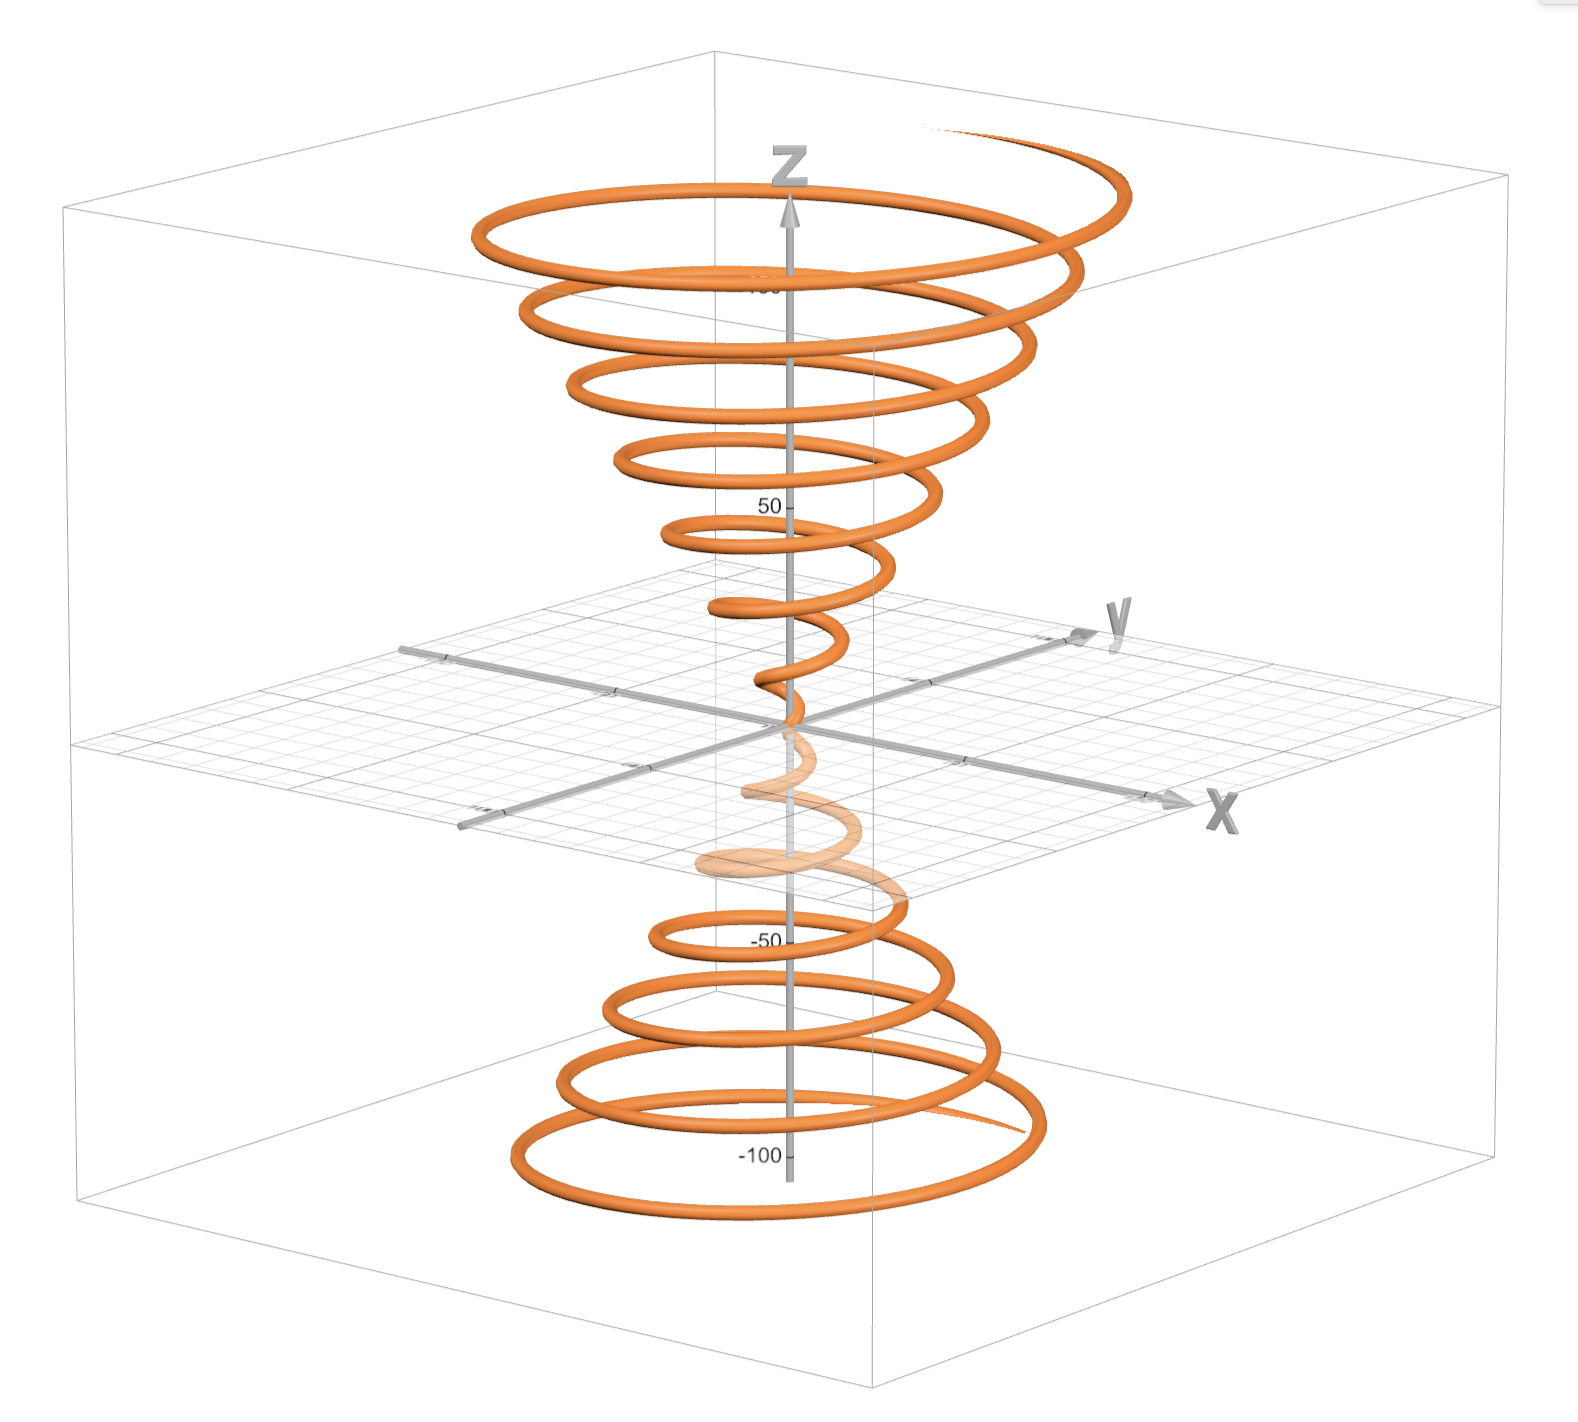
\includegraphics[width=0.32\textwidth]{images/unbounded_spiral.png}
    \caption{Unbounded Conical Spiral.}
    \vspace*{-15pt}
\end{wrapfigure}
\begin{enumerate}[leftmargin=!, itemindent=-5ex]
    \item \textbf{The Christmas tree is “ideal”} -- The Christmas tree is modelled as a \emph{cone}, based on the assumption that an “ideal” tree would be radially symmetrical all around and that the slant of the tree is a straight line.
    \item \textbf{The garland wraps uniformly} -- This means that it wraps in a perfect spiral around the tree, without sagging. The garland should also wrap around the tree with equal spacing between subsequent rotations. Since the tree is approximated to be a cone, the garland wrapping around the tree can be modelled as a \emph{circular conical spiral}.
\end{enumerate}
The following input parameters will be considered for the calculations (visualized in Figure \ref{fig:params}):

\noindent
\begin{minipage}{0.57\textwidth}
    \setlength{\parindent}{17pt}
    \begin{table}[H]
        \centering
        \singlespacing
        \begin{tabularx}{0.9\textwidth}{>{\hsize=0.4\hsize}c>{\hsize=0.6\hsize}X}
            \toprule
            {\bfseries Parameter} & {\bfseries Description}                                          \\
            \midrule
            $H$                   & height of the tree                                               \\
            $R$                   & radius of the based of the tree                                  \\
            $\lambda$             & slant distance (spacing) between successive rotations of garland \\
            \bottomrule
        \end{tabularx}
    \end{table}

    Diagrams and graphs will be used throughout the paper to aid in the explanation of concepts, and unless otherwise mentioned, they are generated using the online graphing calculator \emph{Desmos}.
\end{minipage}
\begin{minipage}{0.4\textwidth}
    \centering
    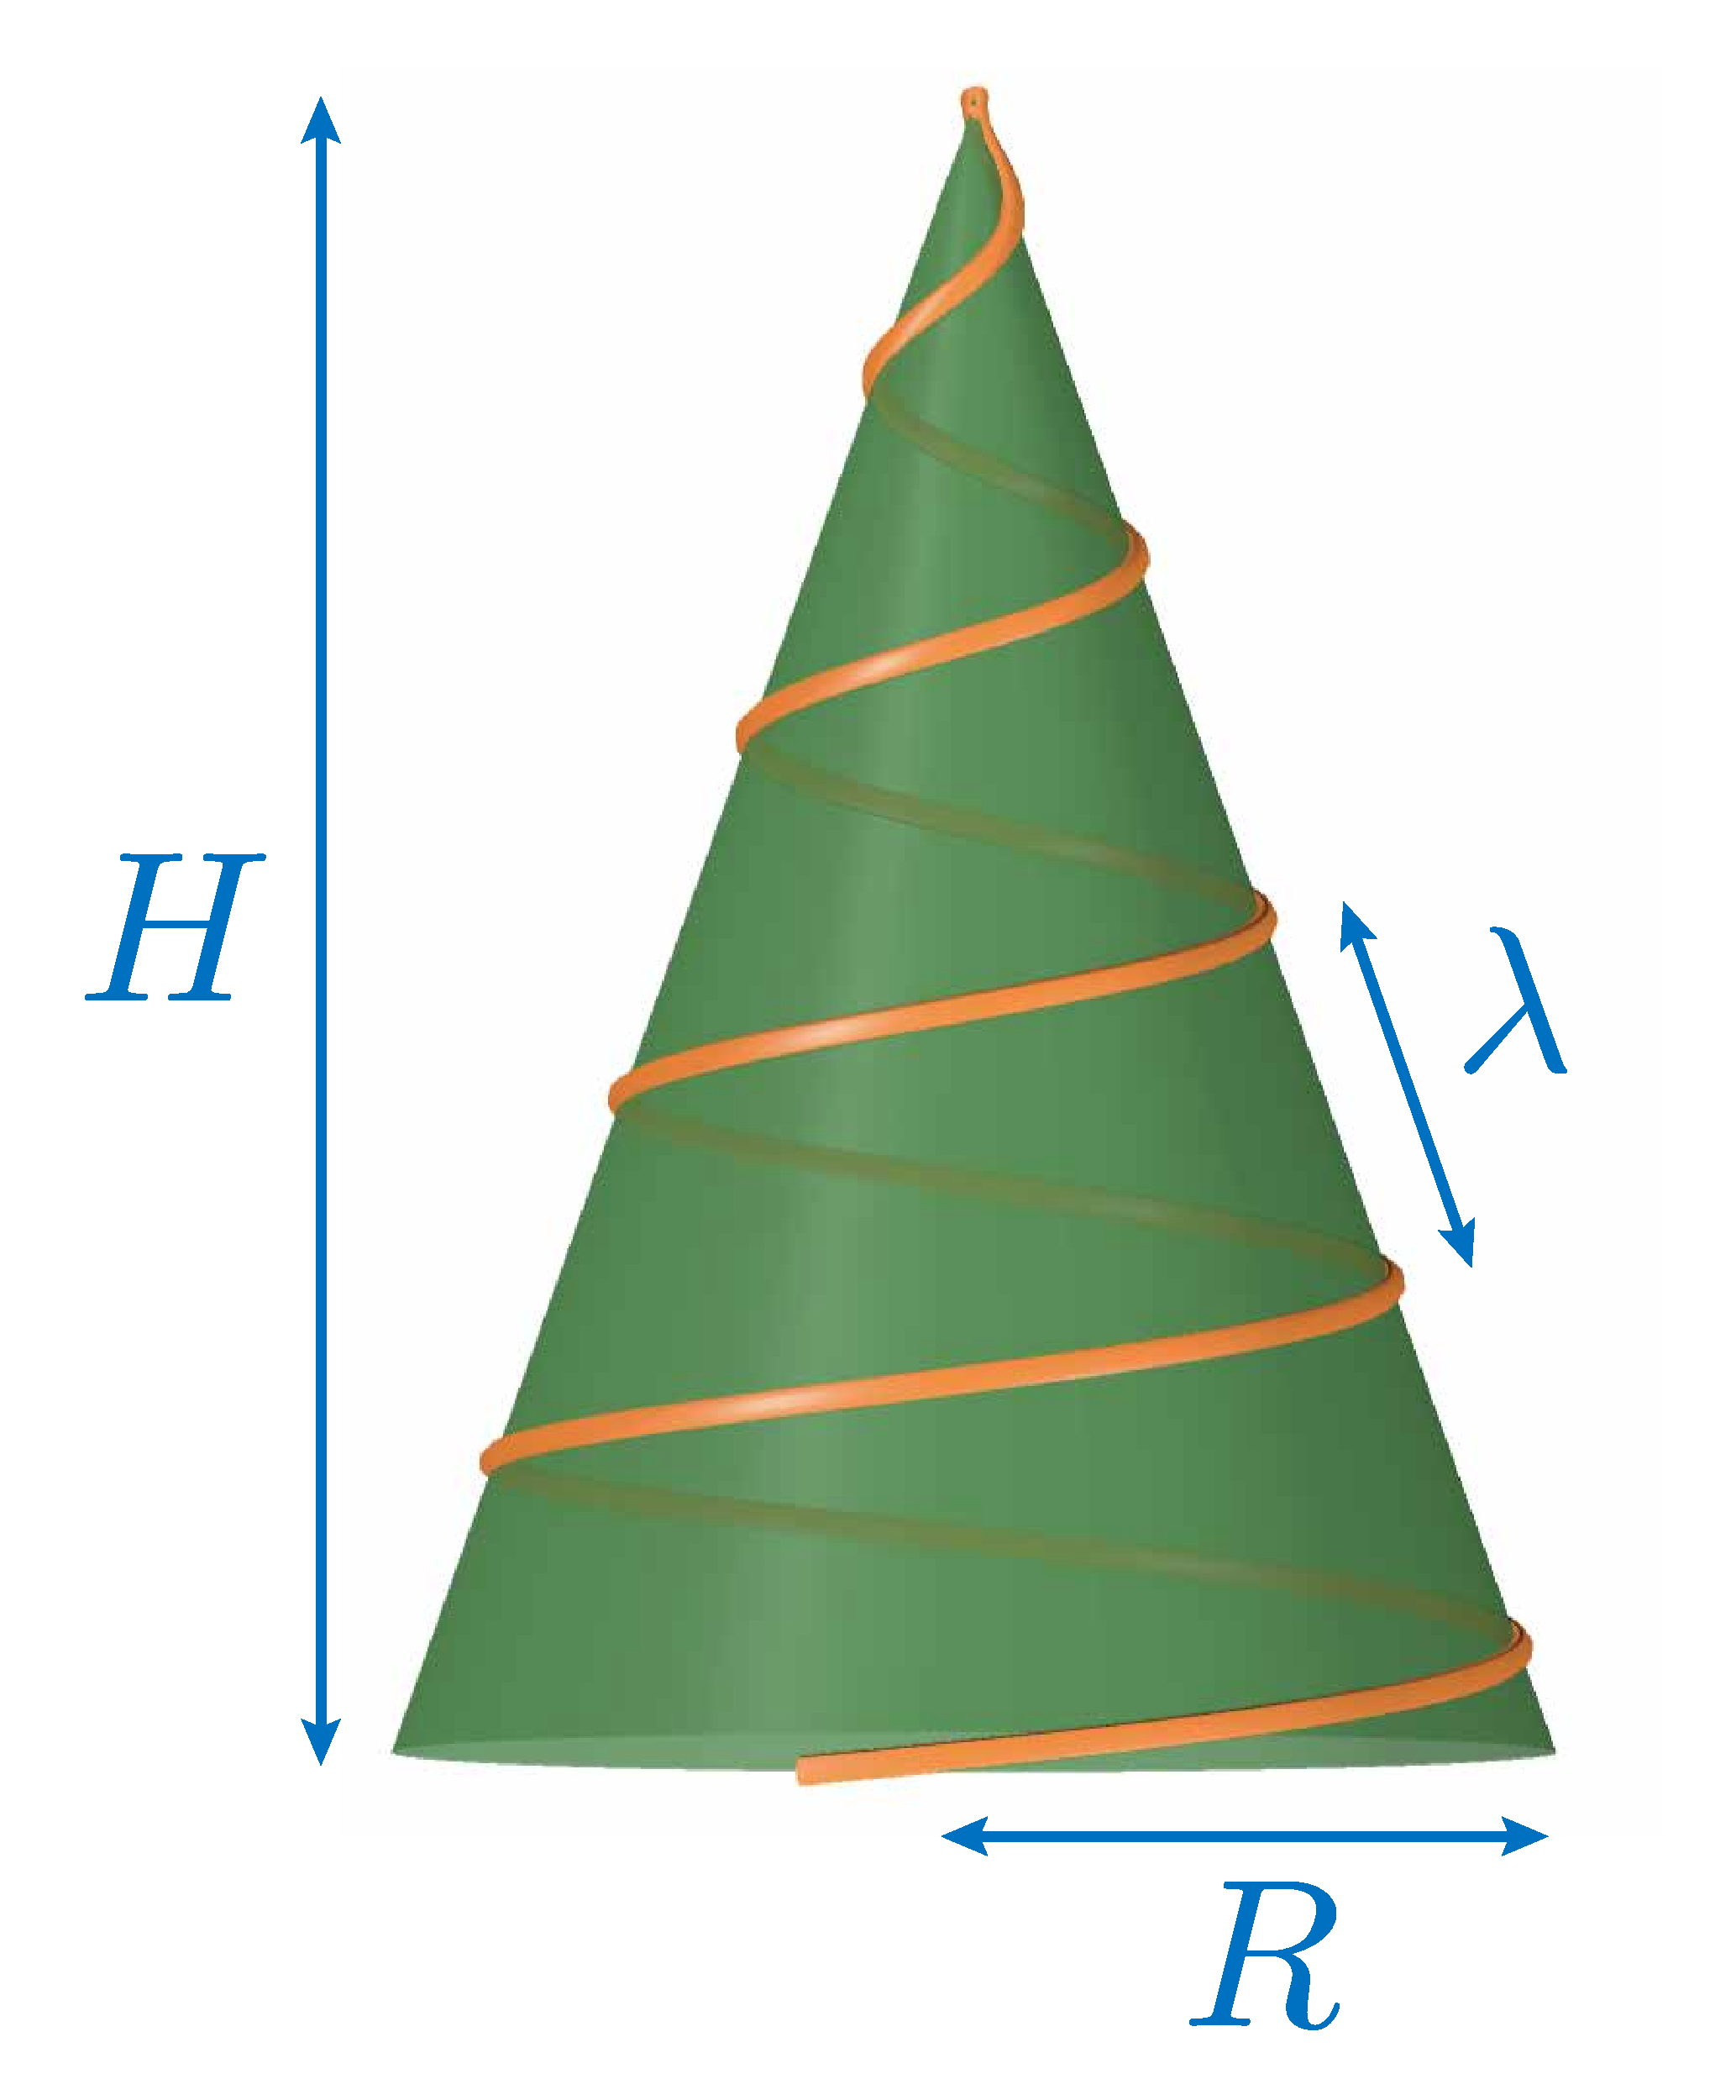
\includegraphics[width=0.9\textwidth]{diagrams/parameters.pdf}
    \captionof{figure}{Input Parameters.} \label{fig:params}
\end{minipage}



\section*{Modelling the Garland}

The garland can be modelled as a circular conical spiral, and applying lower and upper bounds, it has the parametric function \autocite{rejbrandConicalHelix}:
\begin{equation}
    C(t) = \begin{pmatrix}[0.7]
        at\cos{t} \\
        at\sin{t} \\
        bt
    \end{pmatrix}, \quad \forall t \in \left[0, \frac{H}{b}\right]
\end{equation}
where the constants $a, b \in \Real$. Lower and upper bounds are applied because the cone has height $H$, and we only want parts of the curve where $z(t)$ is between $0$ and $H$. Thus, $0 \leq bt \leq H$, and dividing by $b$, we find that $0 \leq t \leq \frac{H}{b}$, which are the bounds applied to $C(t)$. $t$ is the independent variable, and for any given value of $t$, the parametric function outputs a point on the curve, and as we generate an infinite
amount of points from the lower bound to the upper bound, the locus of points formed generate the shape of the space curve. The z-axis of the spiral coincides with the tree's axis of radial symmetry and $C(0)$ represents the tip of the tree.

To ensure that the spiral sits on the surface of the cone (the Christmas tree), it is necessary to find appropriate values for $a$ and $b$. Using methodology inspired by a blog post authored by Stewart and Heighway, we first define the radial distance $\rho(t)$ as the distance of a point on the curve to the tree's axis of radial symmetry, visualized in Figure \ref{fig:radial}. By Pythagorean's theorem:
\begin{equation*}
    \rho(t) = \sqrt{x(t)^2+y(t)^2}
\end{equation*}
\begin{wrapfigure}{r}{0.4\textwidth}
    \centering
    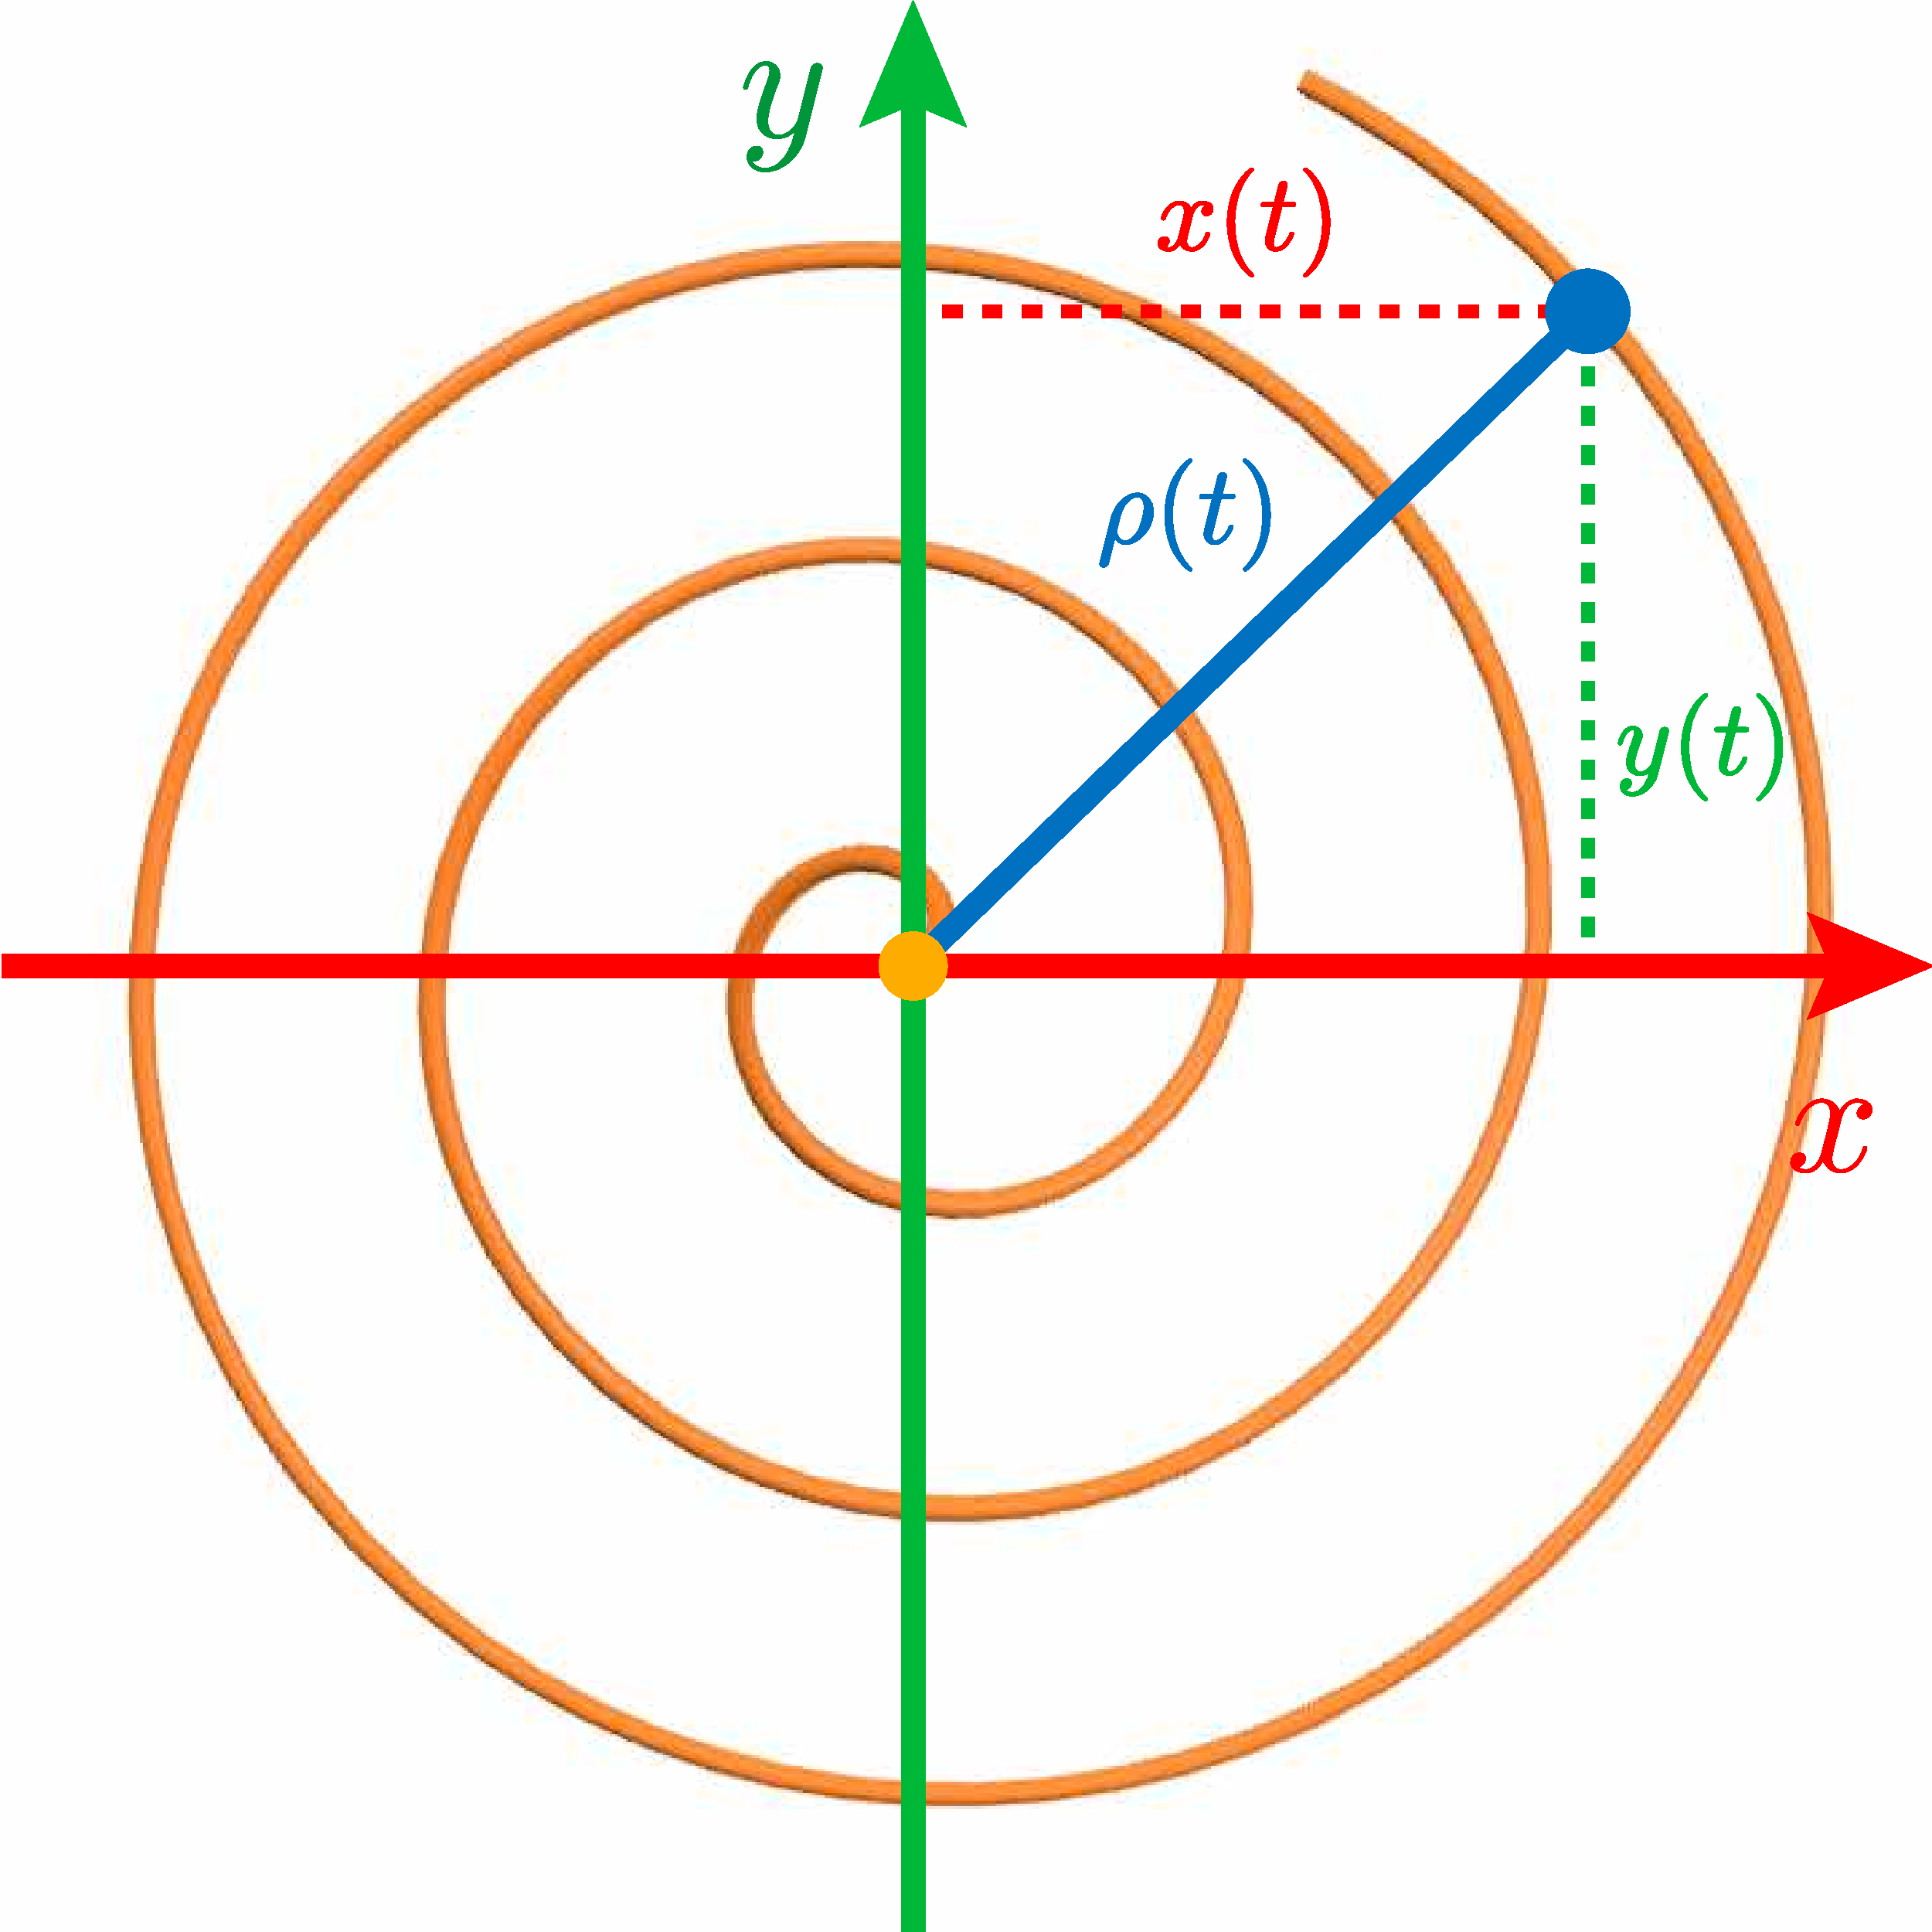
\includegraphics[width=0.38\textwidth]{diagrams/radial_distance.pdf}
    \caption{Radial distance of a point on the spiral to the z-axis (top-down view).} \label{fig:radial}
    \vspace*{-30pt}
\end{wrapfigure}
\bulletarrow Substituting for $x(t)$ and $y(t)$:
\begin{align}
    \rho(t) & = \sqrt{a^2t^2\cos^2{t}+a^2t^2\sin^2{t}} \notag \\
            & = at\sqrt{\cos^2{t}+\sin^2{t}} \notag           \\
            & = at
\end{align}

The radial distance is useful because the ratio of $\rho(t)$ over $z(t)$ for any given $t$ will always be proportional to $H$ over $R$ for any given $t$. This because any valid point of the curve should sit on the surface of the cone of height $H$ and radius $R$, and thus the radial distance $\rho(t)$ and vertical distance $z(t)$ of the point would form a right triangle as visualized in Figure \ref{fig:sim_tri}, which would be similar to the triangle formed by the vertical cross-section of the cone by angle-angle, due to the shared an interior angle. This allows us to establish the following proportional relationship:
\begin{gather}
    \frac{R}{H} = \frac{\rho(t)}{z(t)} = \frac{at}{bt} \notag \\
    \Rightarrow \frac{R}{H} = \frac{a}{b} \label{eq:proportion}
\end{gather}

\begin{wrapfigure}[7]{l}{0.3\textwidth}
    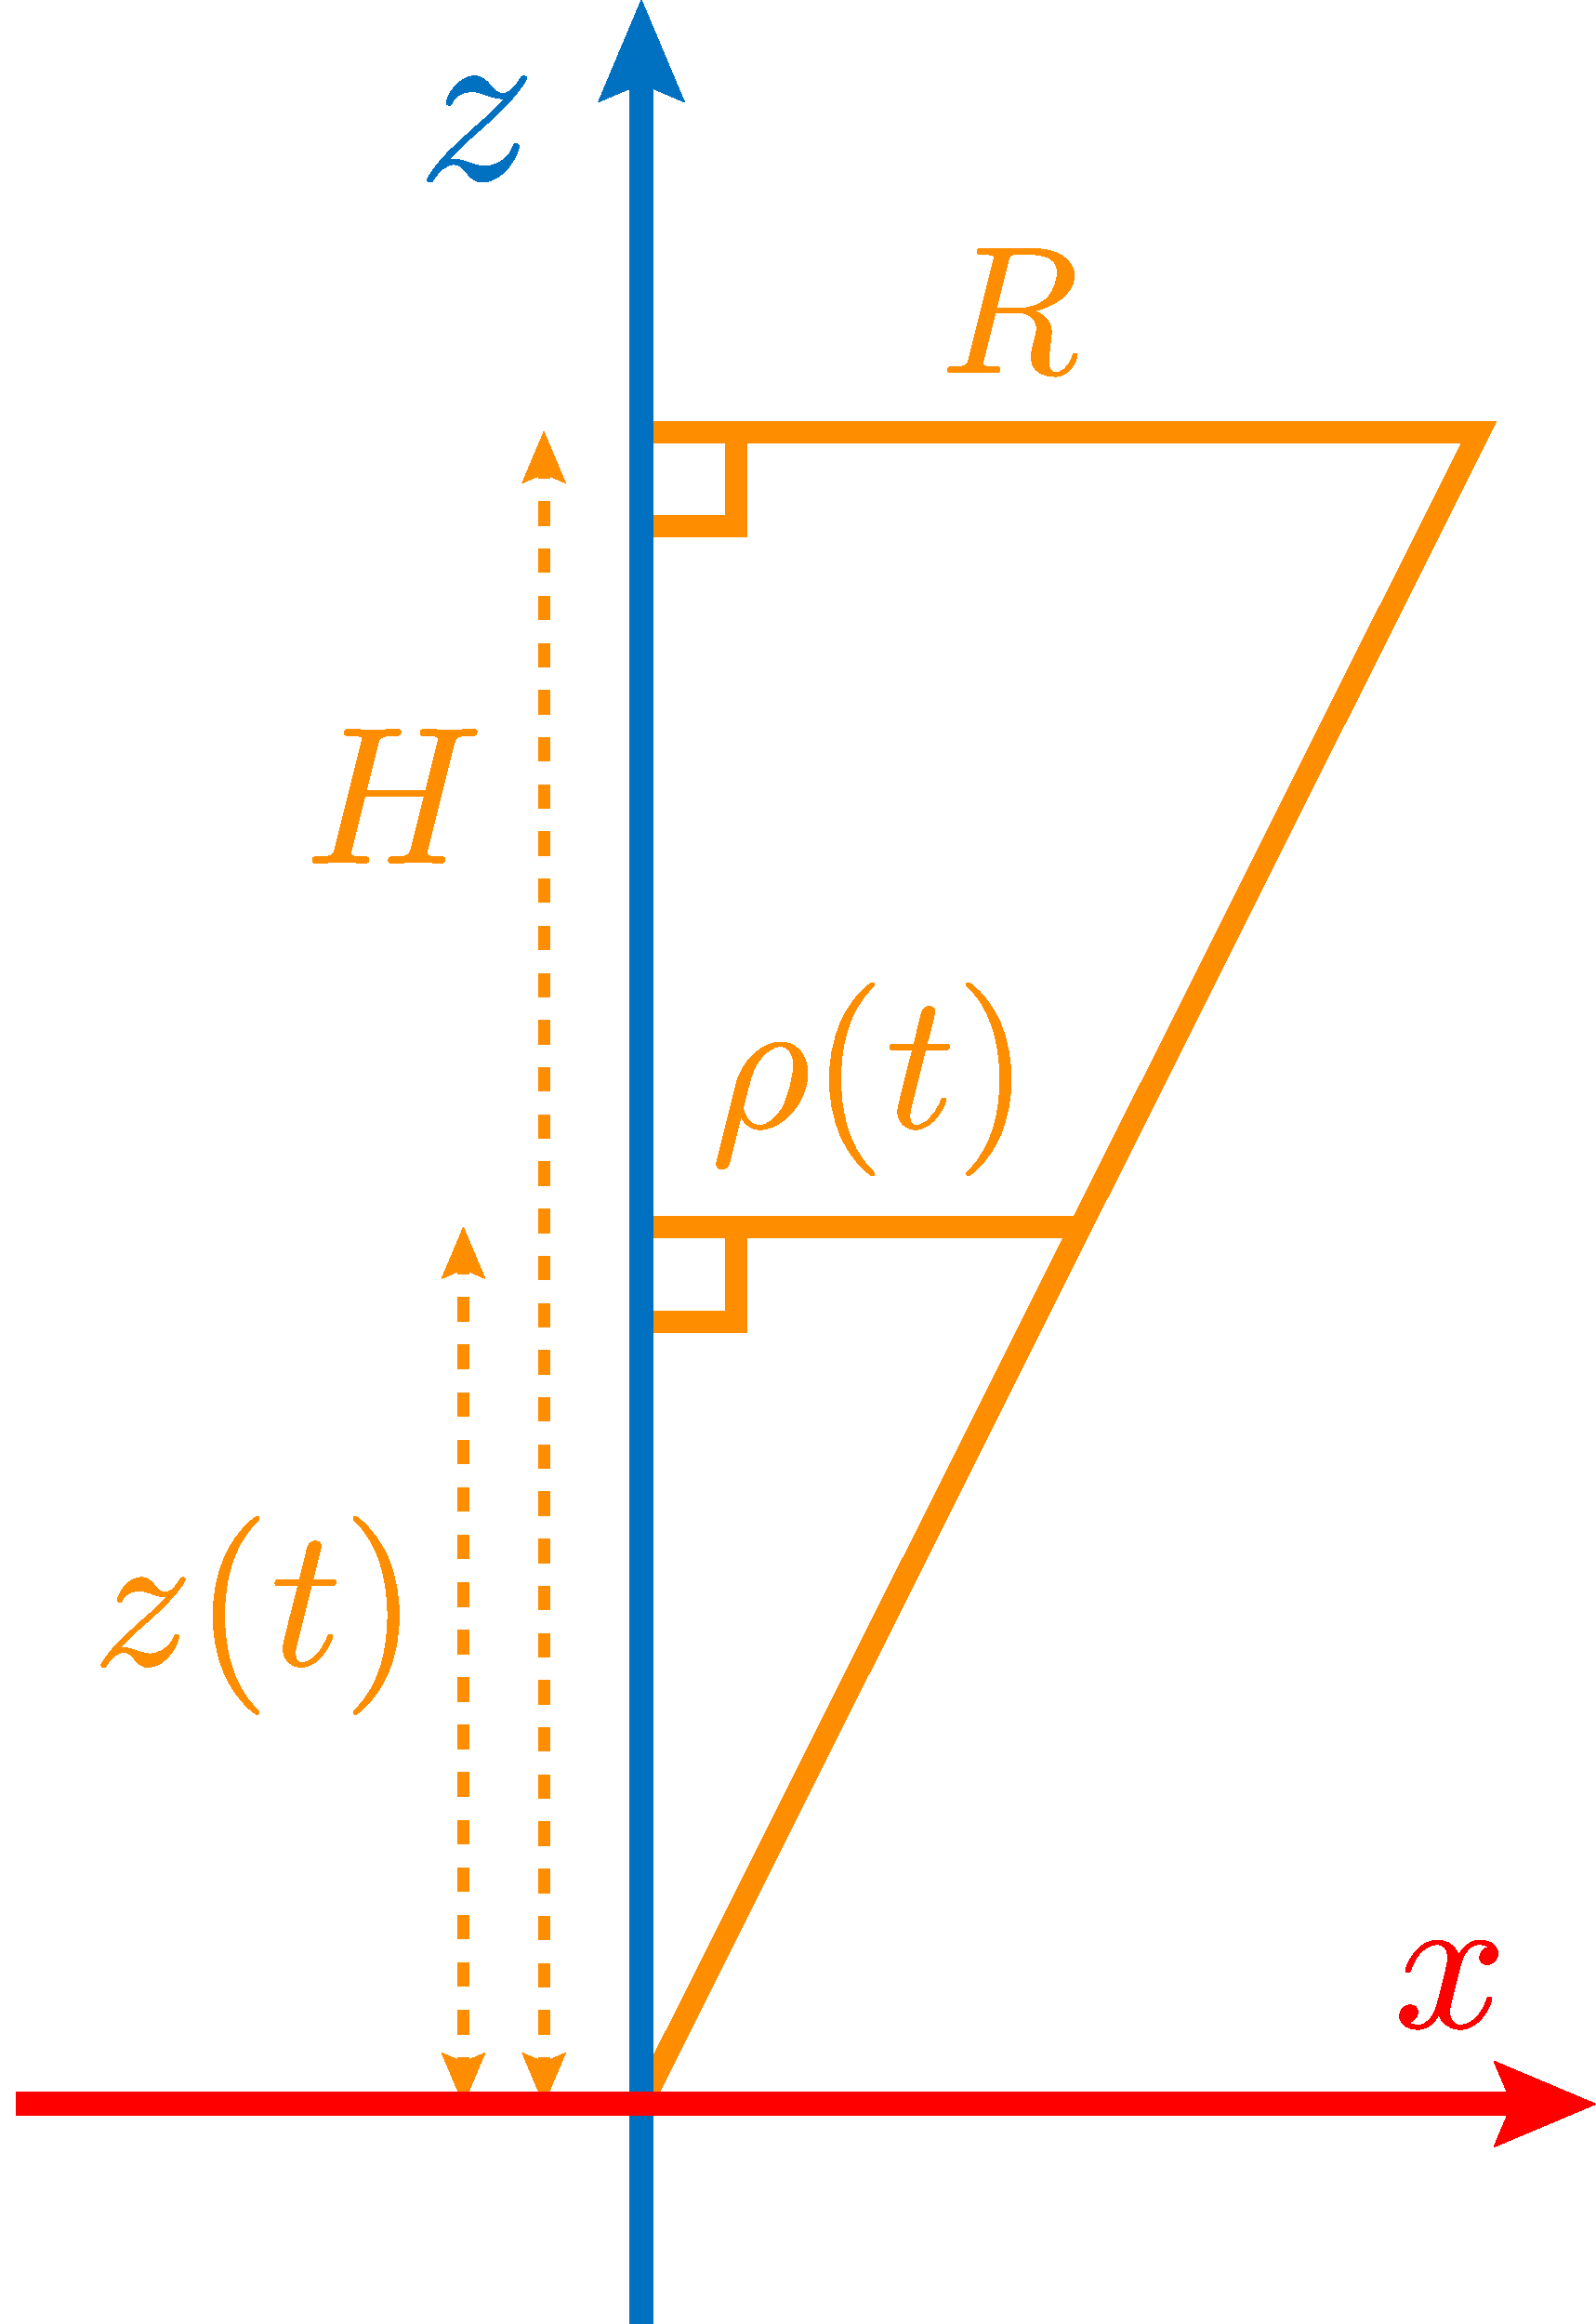
\includegraphics[width=0.28\textwidth]{diagrams/similar_triangles.pdf}
    \caption{Similar Triangles.} \label{fig:sim_tri}
\end{wrapfigure}
In other words, for the spiral to lie on the surface of the cone with radius $R$ and height $H$, the ratio $a$ over $b$ must be proportional to $R$ over $H$. This relationship is visualized in Figure \ref{fig:param_comparison}, where we can see that larger values for $a$ and $b$ correspond to larger spacing between successive rotations of garland, while smaller values lead to smaller spacing between successive rotations of the garland. From this, we can establish a relationship between $\lambda$, $a$, and $b$.

\begin{figure}[H]
    \centering
    \begin{subfigure}[t]{0.32\textwidth}
        \centering
        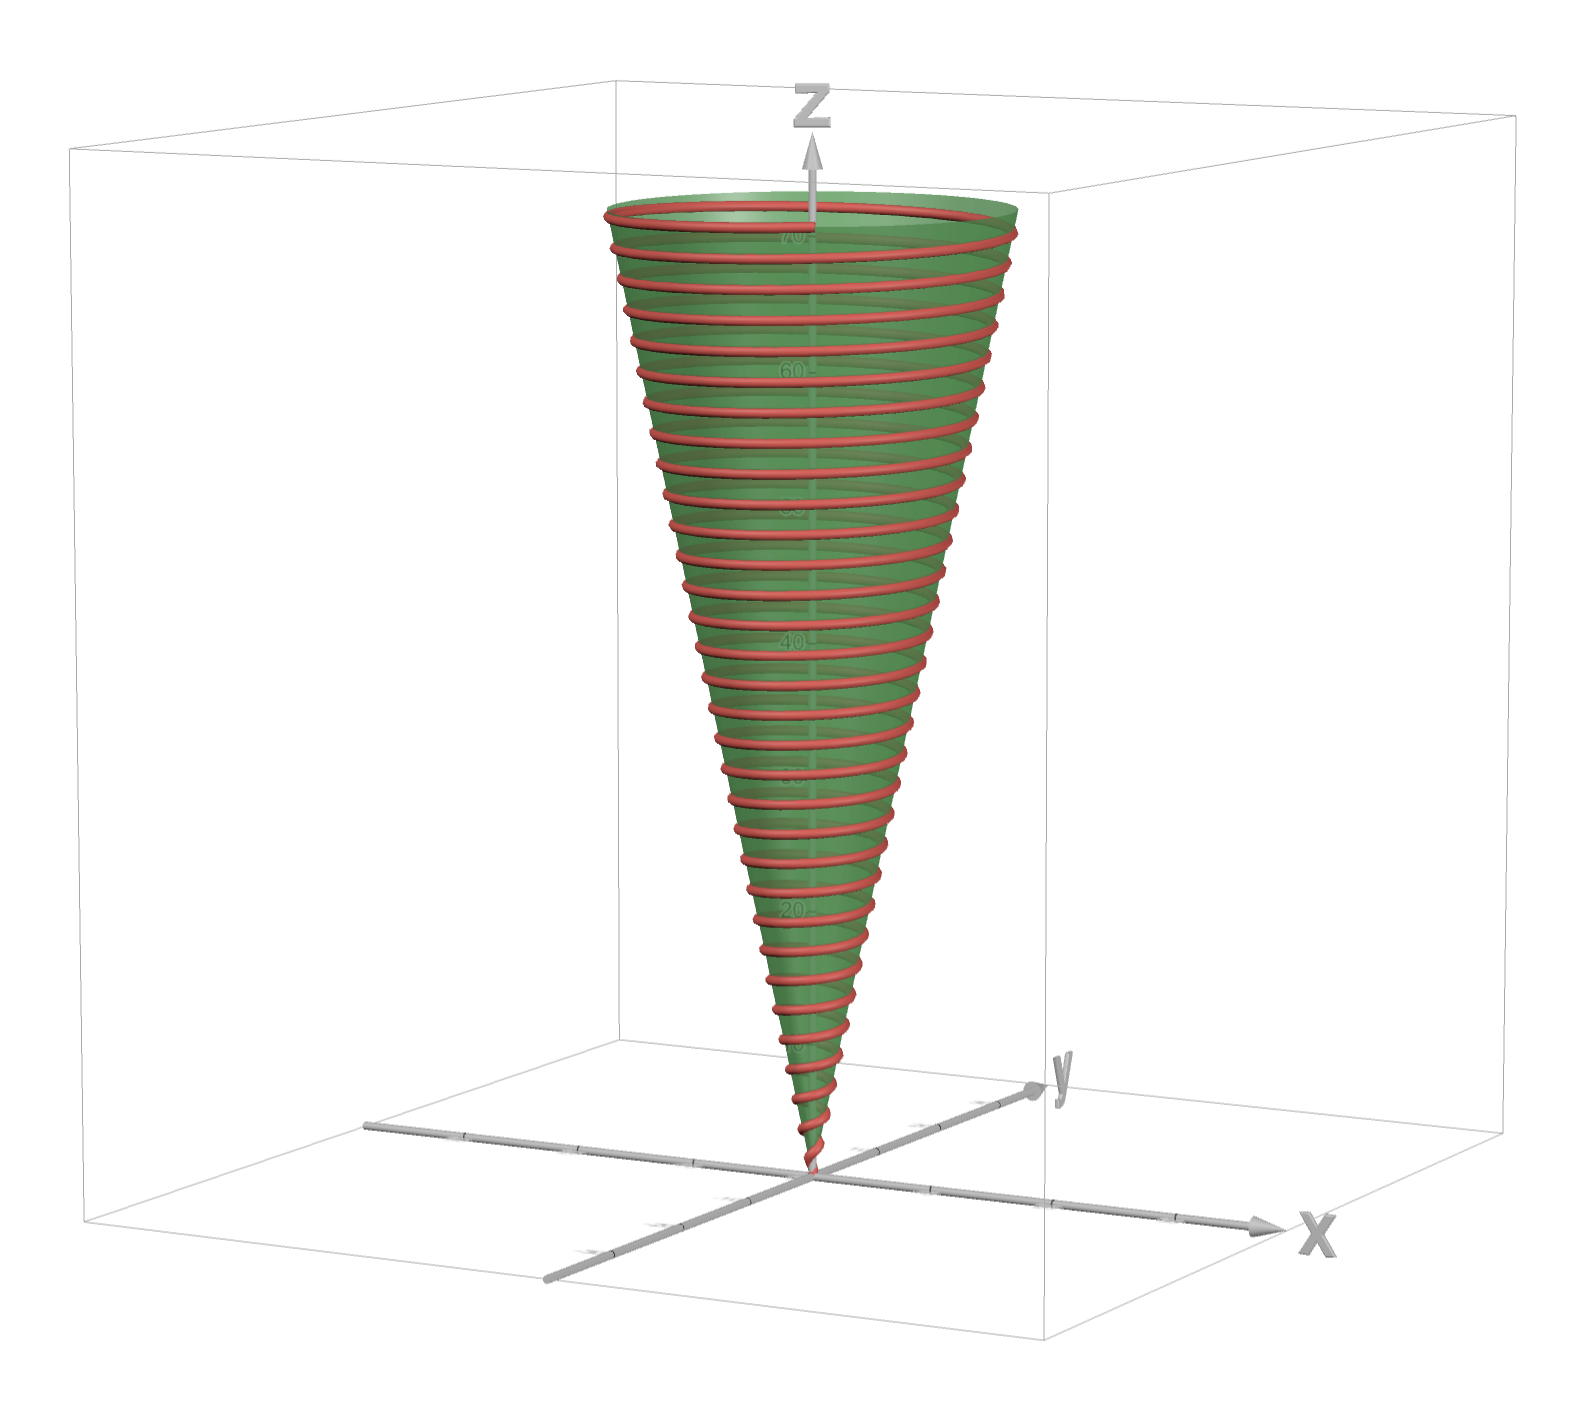
\includegraphics[width=\textwidth]{images/a_vs_b/close.png}
        \caption{$a=0.075$, $b=0.360$}
    \end{subfigure}
    \begin{subfigure}[t]{0.32\textwidth}
        \centering
        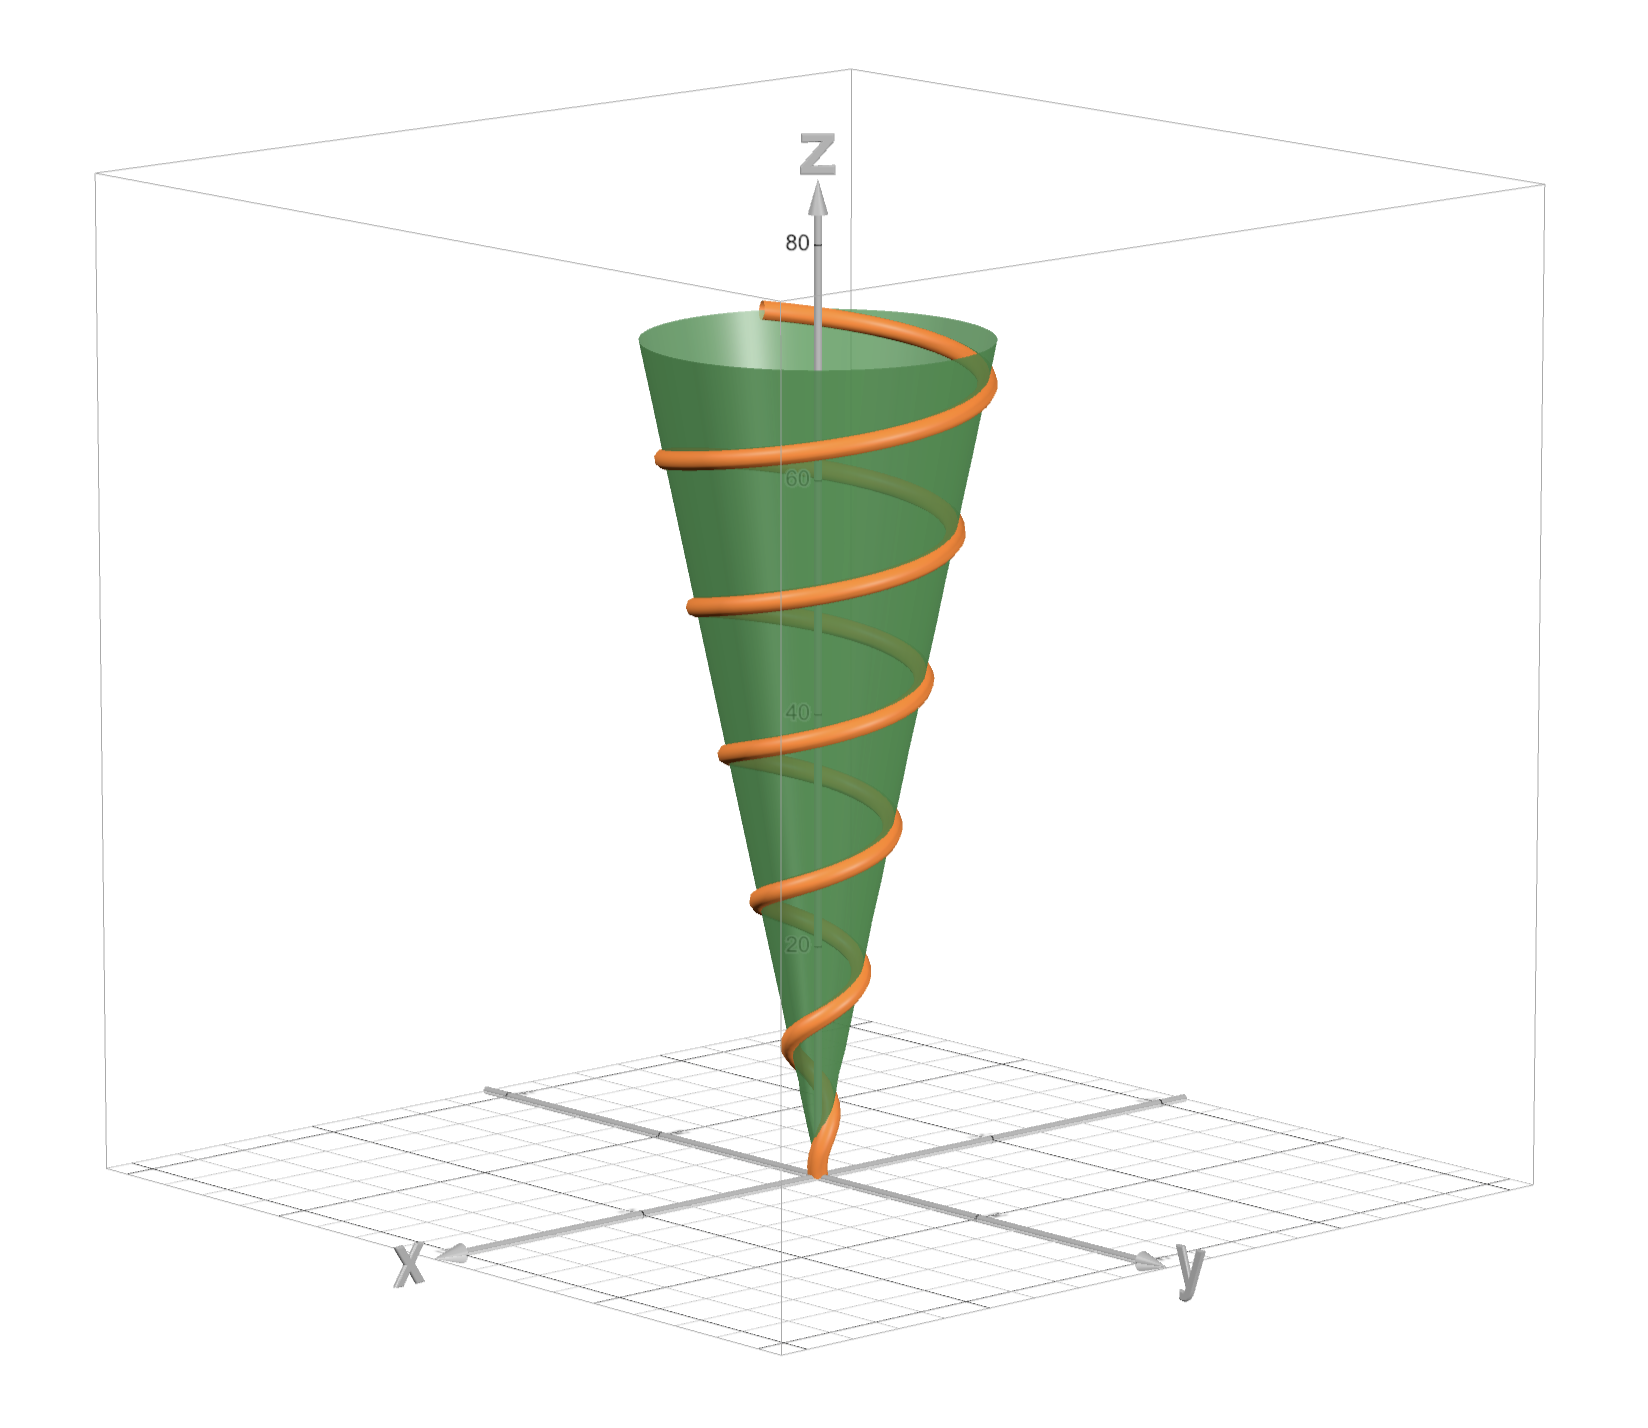
\includegraphics[width=\textwidth]{images/a_vs_b/medium.png}
        \caption{$a=0.225$, $b=1.08$}
    \end{subfigure}
    \begin{subfigure}[t]{0.32\textwidth}
        \centering
        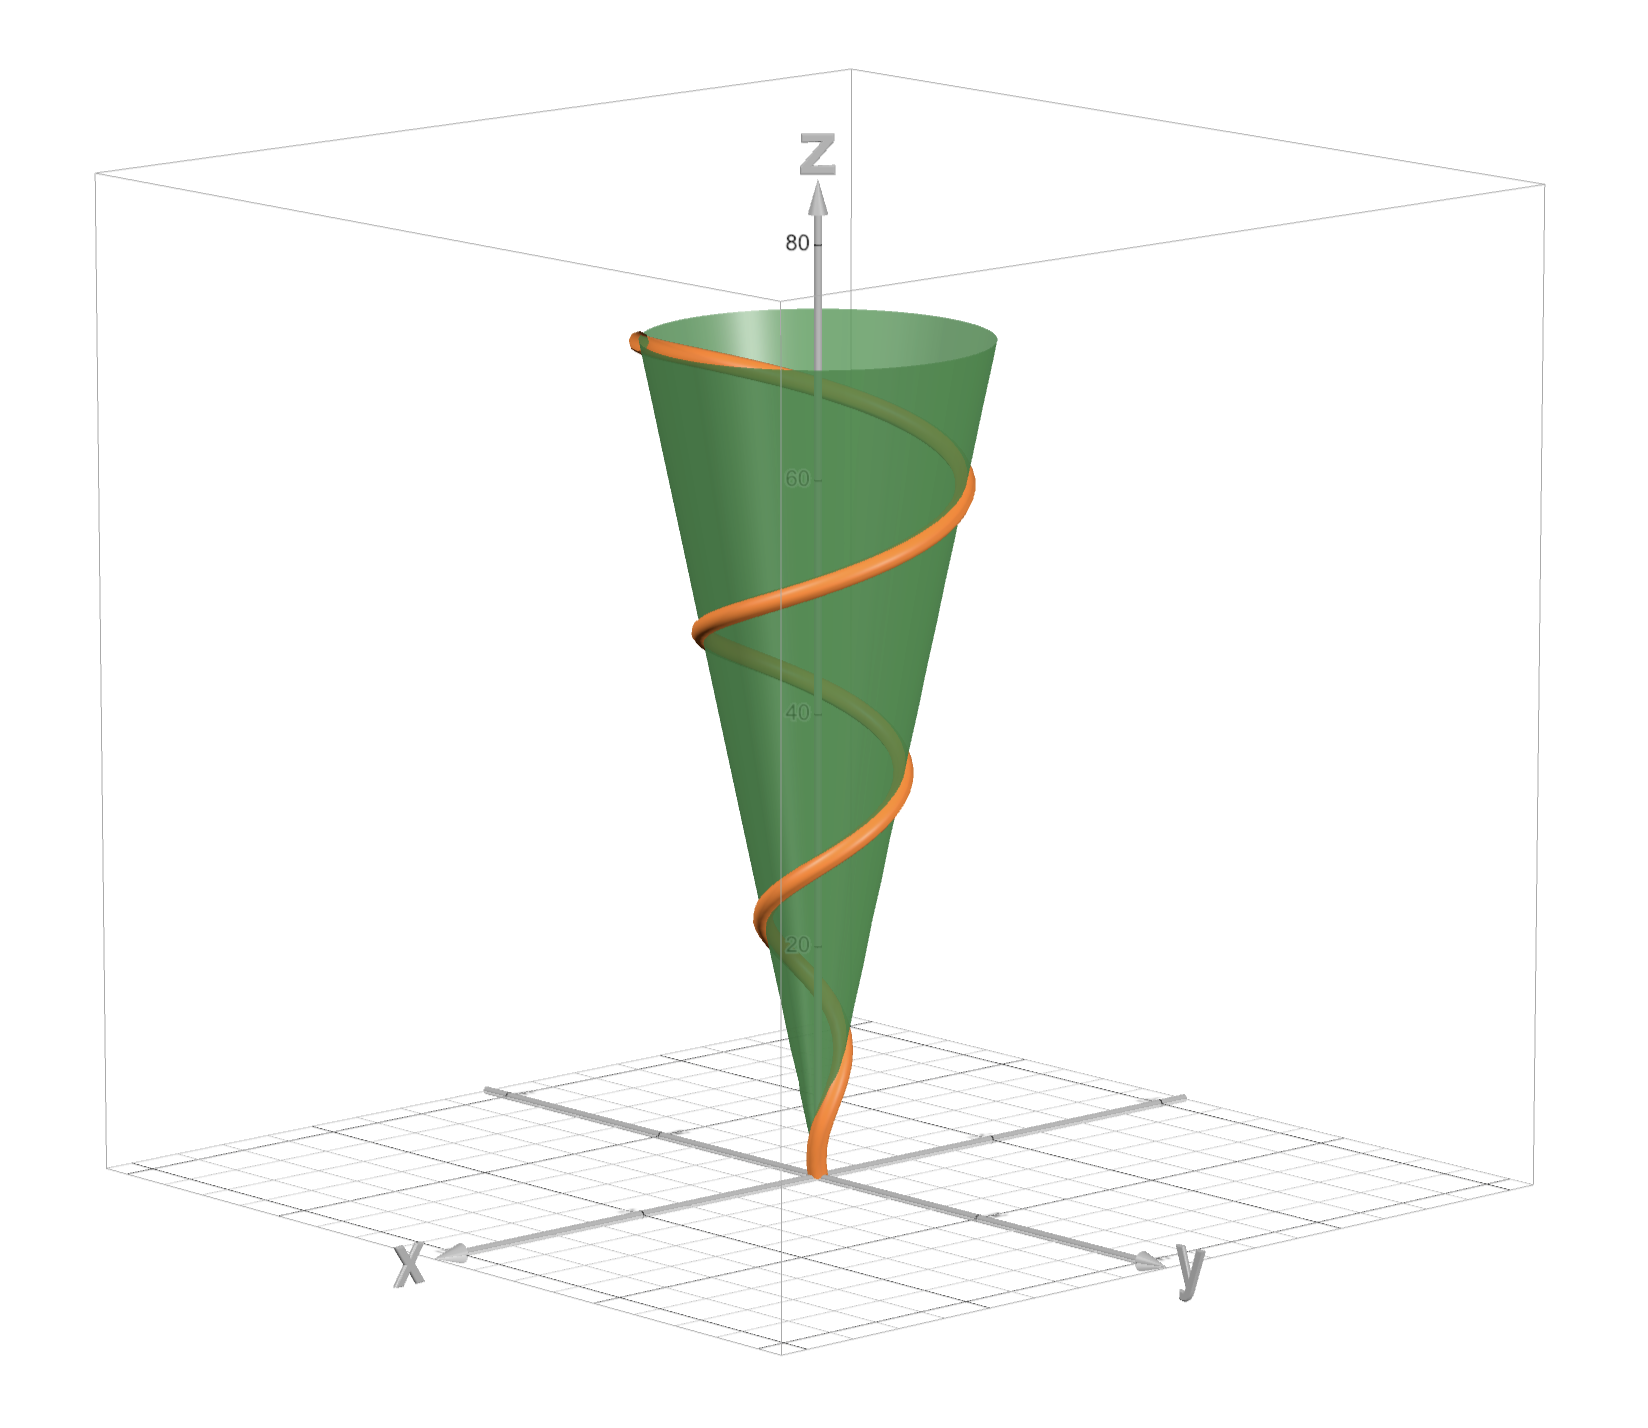
\includegraphics[width=\textwidth]{images/a_vs_b/sparse.png}
        \caption{$a=0.450$, $b=2.16$}
    \end{subfigure}
    \caption{Spirals that have the same ratio of $\frac{a}{b}$ lie on the same cone} \label{fig:param_comparison}
\end{figure}

For every rotation of the garland, $t$ increases by $2\pi$ because that is the period of the trigonometric functions sine and cosine. Thus, the change in radial distance, $\Delta \rho$, and change in vertical distance, $\Delta z$, after one full period would be:
\begin{equation*}
    \begin{aligned}[c]
        \Delta \rho & = \rho(t+2\pi) -\rho(t) \\
                    & = a\cdot(t+2\pi) - at   \\
                    & = 2\pi a
    \end{aligned}
    \qquad\qquad\qquad\qquad
    \begin{aligned}[c]
        \Delta z & = z(t+2\pi) -z(t)     \\
                 & = b\cdot(t+2\pi) - bt \\
                 & = 2\pi b
    \end{aligned}
\end{equation*}
While $\lambda$ represents the distance between consecutive rotations of garland, we can also think of it as the change in position of the spiral along of the slant length of the cone per rotation. Thus, by the Pythagorean theorem:
\begin{equation}
    \lambda^2 = 4\pi^2a^2+4\pi^2b^2 \label{eq:spacing}
\end{equation}
With this, we now have 2 equations with $a$ and $b$, and we can represent $a$ and $b$ in terms of our chosen parameters. From equation \ref{eq:proportion}, we can isolate $b$ to get that $b = \frac{H}{R}a$, which can be substituted back into equation \ref{eq:spacing}:
\begin{equation*}
    \Rightarrow \lambda^2 = 4\pi^2a^2+\frac{4\pi^2a^2H^2}{R^2}  = 4\pi^2a^2\left(1+\frac{H^2}{R^2} \right)
\end{equation*}
\bulletarrow Isolating for $a$:
\begin{equation*}
    a = \sqrt{\frac{\lambda^2}{4\pi^2(1+\frac{H^2}{R^2})}} = \frac{\lambda}{2\pi\sqrt{1+\frac{H^2}{R^2}}} = \frac{\lambda R}{2\pi\sqrt{R^2+H^2}}
\end{equation*}
\bulletarrow Recognizing that $S=\sqrt{R^2+H^2}$ is the slant height of the cone:
\begin{equation}
    a =\frac{\lambda R}{2\pi S}
\end{equation}
\bulletarrow Plugging this back in equation \ref{eq:proportion}, we get:\begin{equation}
    b =\frac{\lambda H}{2\pi S}
\end{equation}
Thus, we finally have that the parametric equation for the garland is:
\begin{equation}
    C(t) = \frac{\lambda}{2\pi S}
    \begin{pmatrix}[0.7]
        Rt\cos{t} \\
        Rt\sin{t} \\
        Ht
    \end{pmatrix}, \quad \forall t \in \left[0, \frac{2\pi S}{\lambda}\right]
\end{equation}

\section*{Deriving an Equation for the Length of the Garland}

With a function which models the garland, we can now calculate the length of the garland by calculating the \emph{arc length} of $C(t)$. The arc length, $L$, is defined as the distance travelled along the path of a curve from one point to another \autocite{ArcLength2017}. The arc length of $C(t)$ can be evaluated by decomposing the curve into an infinite amount of infinitesimally small line segments, $\dd{L}$, and adding their lengths. Thus, the length of the garland is represented by the definite integral:
\begin{equation}
    L=\int_0^\frac{2\pi S}{\lambda} \dd{L} \label{eq:arclen}
\end{equation}

The lower and upper bounds on the integral are a result of the restrictions imposed on $C(t)$.

\begin{wrapfigure}{r}{0.35\textwidth}
    \centering
    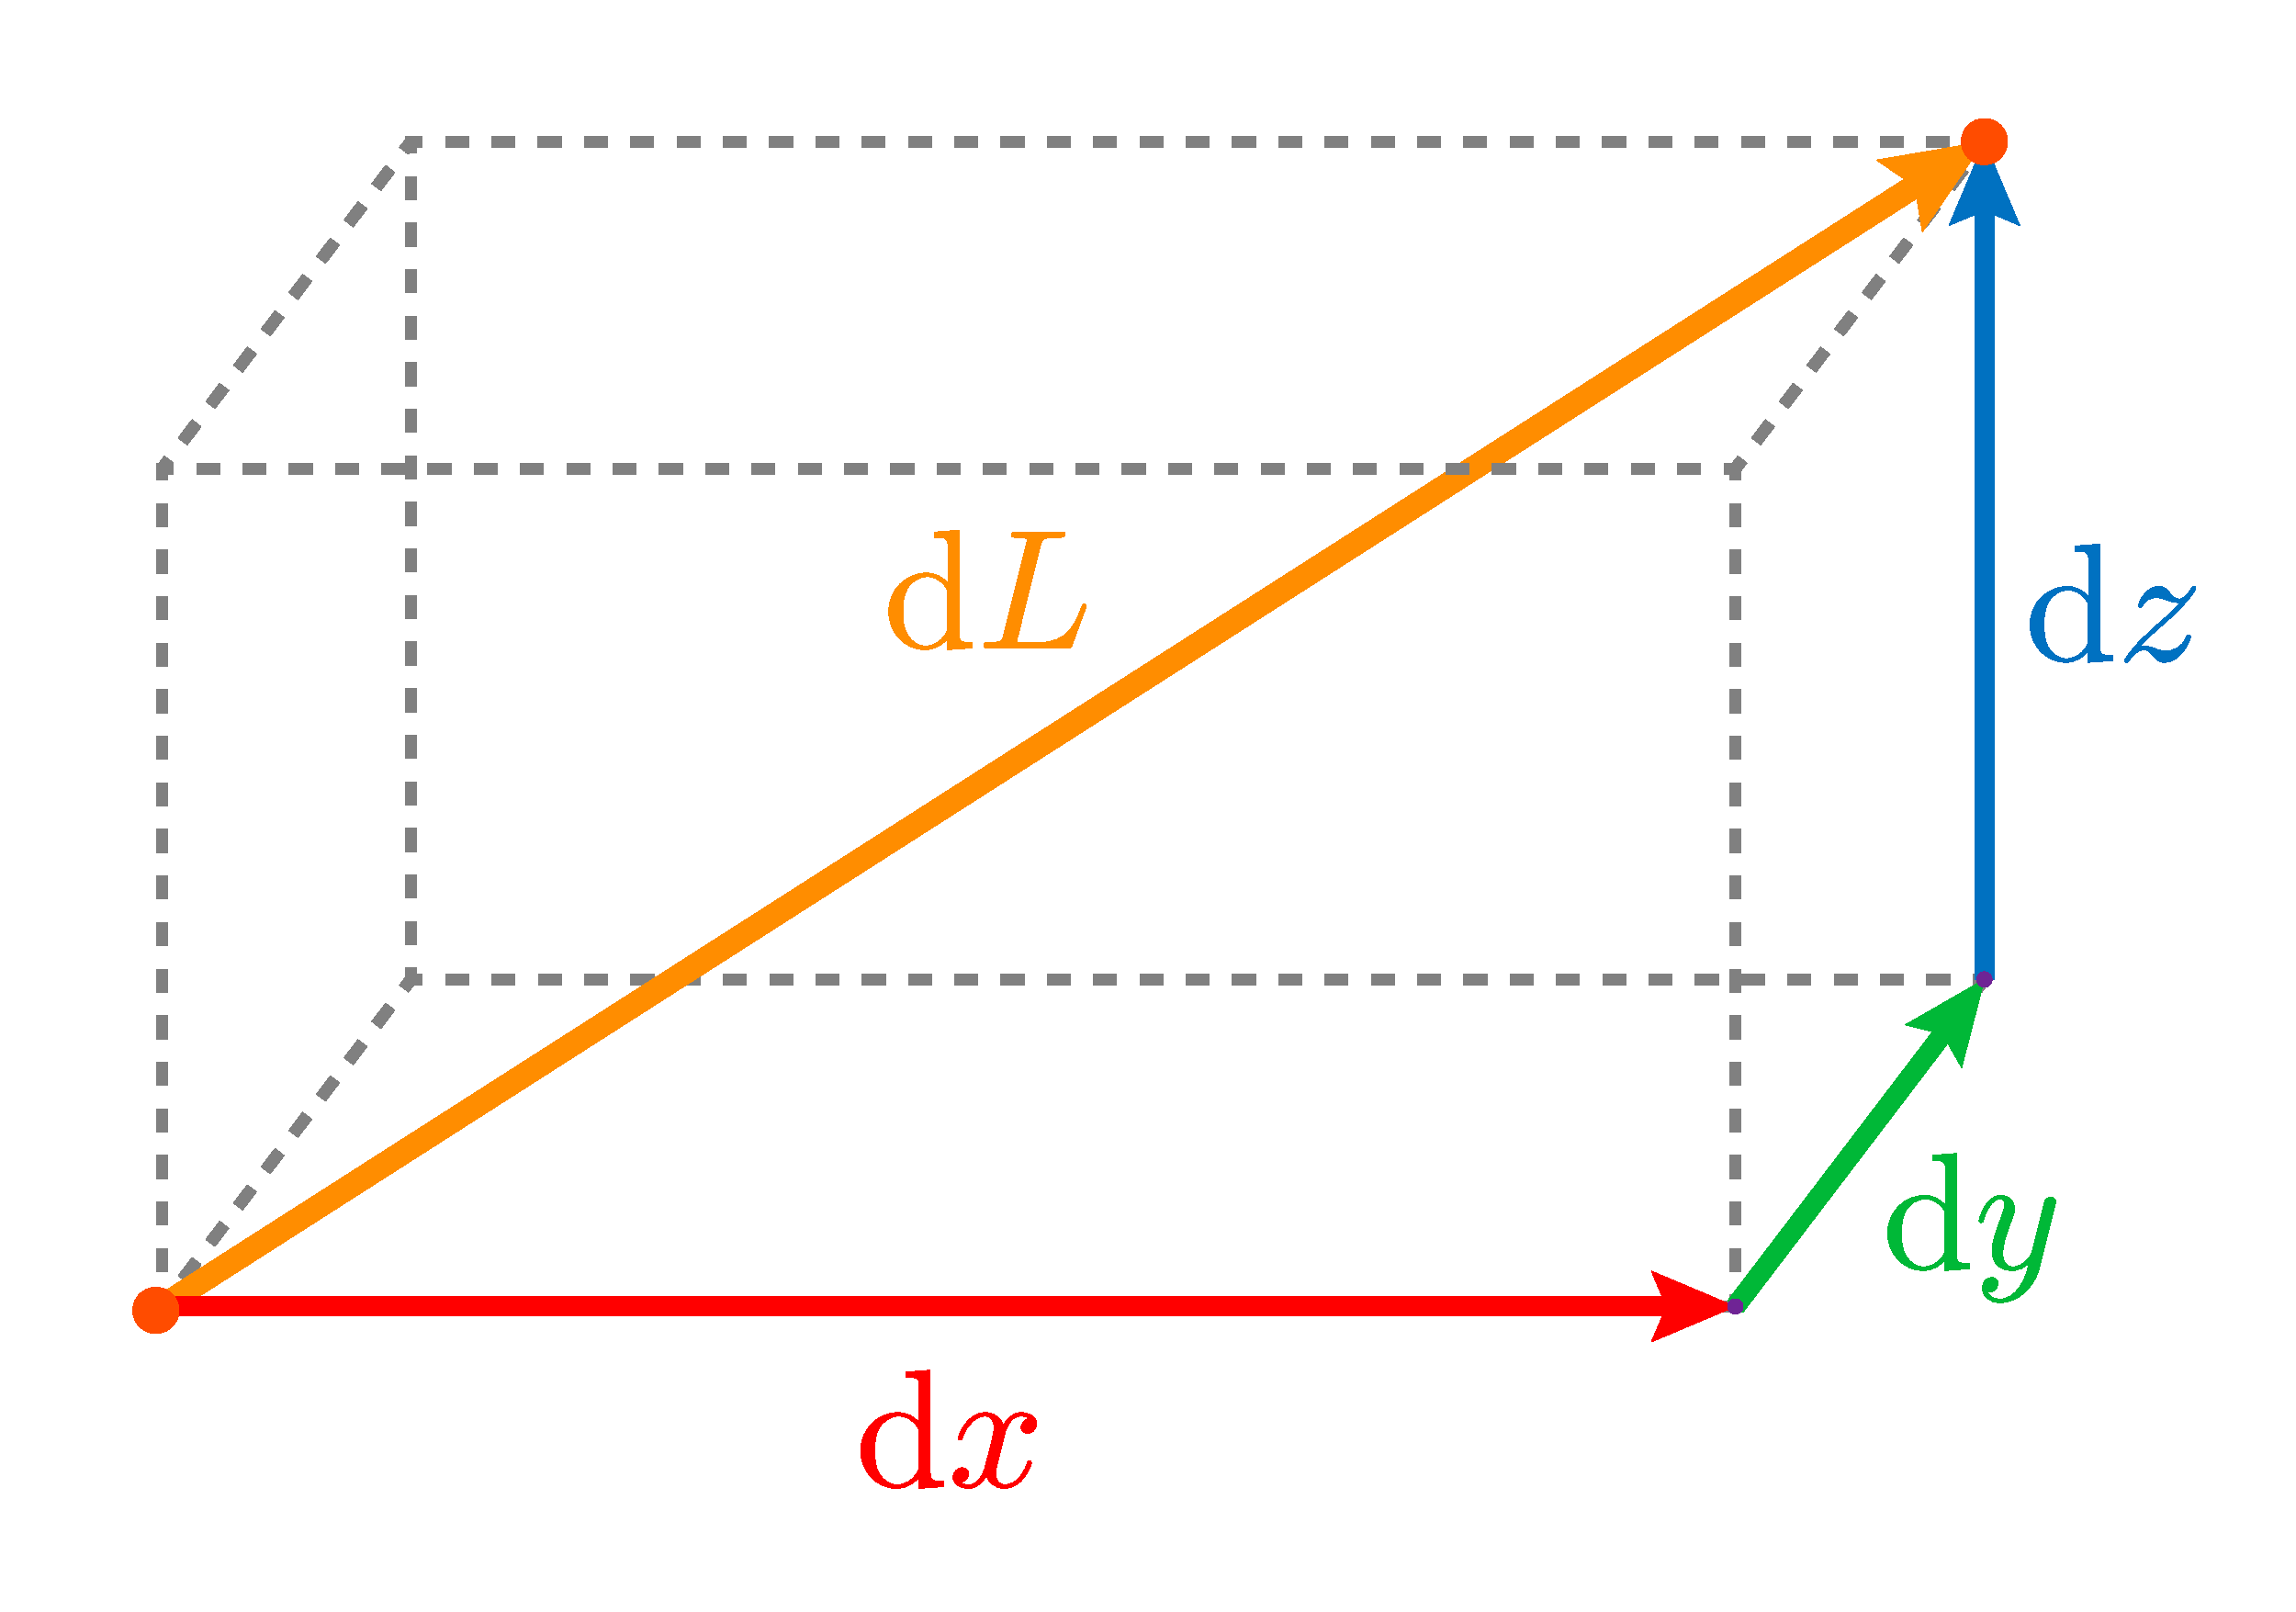
\includegraphics[width=0.32\textwidth]{diagrams/dL.pdf}
    \caption{$\dd{L}$ in terms of $\dd{x}$, $\dd{y}$, and $\dd{z}$} \label{fig:dL}
\end{wrapfigure}
However, what is $\dd{L}$? To find what $\dd{L}$ is, it is useful to think of it as a 3-dimensional vector. One important property of vectors is that they can be expressed as a sum of multiple vectors, and thus 3D vectors can be decomposed into their $x$, $y$, and $z$  components. Using this line of thinking, it can similarly be said that $\dd{L}$ can be
decomposed into the infinitesimals $\dd{x}$, $\dd{y}$, and $\dd{z}$, as visualized in Figure \ref{fig:dL}. Therefore, applying the 3D Pythagorean theorem:
\begin{equation*}
    \dd{L} = \sqrt{(\dd{x})^2+(\dd{y})^2+(\dd{z})^2}
\end{equation*}

However, this is not of much use, as $\dd{x}$, $\dd{y}$, and $\dd{z}$ are arbitrary. Thus, $\dd{t}$ is introduced into the equation by multiplying the equation by $\frac{\dd{t}}{\dd{t}}$, and with some algebraic manipulation, $\dd{L}$ can be expressed in terms of the derivatives of $x(t)$, $y(t)$, and $z(t)$ components of the curve, which can be easily evaluated \autocite{schlickerArcLength}:
\begin{equation*}
    \dd{L} = \sqrt{\frac{(\dd{x})^2+(\dd{y})^2+(\dd{z})^2}{(\dd{t})^2}} \cdot \dd{t} = \sqrt{\left(\dv{x}{t}\right)^2+\left(\dv{y}{t}\right)^2+\left(\dv{z}{t}\right)^2} \cdot \dd{t}
\end{equation*}
\bulletarrow Substituting in $x(t)$, $y(t)$, and $z(t)$:
\begin{align*}
    \Rightarrow \dd{L} & = \sqrt{\left(\dv{t}\left(\frac{\lambda}{2\pi S}Rt\cos{t}\right)\right)^2+\left(\dv{t}\left(\frac{\lambda}{2\pi S}Rt\sin{t}\right)\right)^2+\left(\dv{t}\left(\frac{\lambda}{2\pi S}Ht\right)\right)^2} \cdot \dd{t} \\
           &= \frac{\lambda}{2\pi S}\sqrt{\left(\dv{t}\left(Rt\cos{t}\right)\right)^2+\left(\dv{t}\left(Rt\sin{t}\right)\right)^2+\left(\dv{t}\left(Ht\right)\right)^2} \cdot \dd{t} \\
           &= \frac{\lambda}{2\pi S}\sqrt{(R\cos{t}-Rt\sin{t})^2+(R\sin{t}-Rt\cos{t})^2+H^2} \cdot \dd{t}
\end{align*}
\bulletarrow Expanding and simplifying:
\begin{align}
    \Rightarrow \dd{L} &= \frac{\lambda}{2\pi S}\sqrt{(R^2\cos^2{t}-\cancel{2R^2t\sin{t}\cos{t}}+R^2t^2\sin^2{t})+(R^2\sin^2{t}+\cancel{2R^2t\sin{t}\cos{t}}+R^2t^2\cos^2{t})+H^2} \cdot \dd{t} \notag \\ 
     &= \frac{\lambda}{2\pi S}\sqrt{R^2(\cancel{\sin^2{t} + \cos^2{t}})+ R^2t^2(\cancel{\sin^2{t}+\cos^2{t}})+H^2} \cdot \dd{t} \notag \\ 
     &= \frac{\lambda}{2\pi S}\sqrt{R^2 +H^2 + R^2t^2} \cdot \dd{t} \notag \\ 
     &= \frac{\lambda}{2\pi S}\sqrt{S^2 + R^2t^2} \cdot \dd{t} 
\end{align}
\bulletarrow Substituting this back into equation \ref{eq:arclen}, we finally obtain:
\begin{equation}
    L = \frac{\lambda}{2\pi S}\int_0^\frac{2\pi S}{\lambda} \sqrt{S^2 + R^2t^2} \cdot \dd{t} \label{eq:integral}
\end{equation}

\section{Evaluating the Integral}
Now, we evaluate the integral so that we can finally obtain a general solution for the length of the garland based on our chosen parameters. Since the integral is of the form $\sqrt{c^2+x^2}$, it can be evaluated using trigonometric substitution.
\newline\bulletarrow{Let $t=\frac{S}{R}\tan{\theta}$. Thus, $\dd{t} = \frac{S}{R}\sec^2{\theta} \dd{\theta}$. Substituting them into equation \ref{eq:integral}:}
\begin{align}
    \Rightarrow L & = \frac{\lambda}{2\pi \cancel{S}}\int_0^{t =\frac{2\pi S}{\lambda}} \sqrt{S^2 + R^2\left(\frac{S}{R}\tan{\theta}\right)^2} \cdot \frac{\cancel{S}}{R}\sec^2{\theta} \dd{\theta} \notag \\
                  & = \frac{\lambda}{2\pi R}\int_0^{t =\frac{2\pi S}{\lambda}} \sqrt{S^2 + S^2\tan^2{\theta}} \cdot \sec^2{\theta} \dd{\theta} \notag                                                      \\
                  & = \frac{\lambda}{2\pi R}\int_0^{t =\frac{2\pi S}{\lambda}} S\sec{\theta} \cdot \sec^2{\theta} \dd{\theta} \notag                                                                       \\
                  & = \frac{\lambda S}{2\pi R}\int_0^{t =\frac{2\pi S}{\lambda}} \sec^3{\theta} \dd{\theta}    \label{eq:subbed}
\end{align}
Then, using integration by parts, the integral of $\sec^3{\theta}$ can be evaluated.
\newline\bulletarrow{Let $u=\sec{\theta}$ and $\dd{v} = \sec^2{\theta} \dd{\theta}$. Therefore, $\dd{u} = \sec{\theta}\tan{\theta}$ and $v = \tan{\theta}$.}
\begin{equation*}
    \Rightarrow L = \frac{\lambda S}{2\pi R}\left[\eval{\sec{\theta}\tan{\theta}}_0^{t =\frac{2\pi S}{\lambda}}-\int_0^{t =\frac{2\pi S}{\lambda}} \sec{\theta}\tan^2{\theta} \dd{\theta}
    \right]
\end{equation*}
\bulletarrow{Using the identity $\tan^2{\theta} = \sec^2{\theta} - 1$:}
\begin{align*}
    \Rightarrow L & = \frac{\lambda S}{2\pi R}\left[\eval{\sec{\theta}\tan{\theta}}_0^{t =\frac{2\pi S}{\lambda}}-\int_0^{t =\frac{2\pi S}{\lambda}} (\sec^3{\theta} - \sec{\theta}) \dd{\theta}\right]                                                                      \\
                  & = \frac{\lambda S}{2\pi R}\left[\eval{\sec{\theta}\tan{\theta}}_0^{t =\frac{2\pi S}{\lambda}}+\int_0^{t =\frac{2\pi S}{\lambda}}  \sec{\theta} \dd{\theta}\right] - \frac{\lambda S}{2\pi R}\int_0^{t =\frac{2\pi S}{\lambda}}\sec^3{\theta} \dd{\theta}
\end{align*}
\bulletarrow{By $\int \sec{\theta} \dd{\theta} = \ln(\sec{\theta}+\tan{\theta})+c$:}
\begin{equation*}
    \Rightarrow L = \frac{\lambda S}{2\pi R}\eval[\sec{\theta}\tan{\theta}+\ln(\sec{\theta}+\tan{\theta})|_0^{t =\frac{2\pi S}{\lambda}} - \frac{\lambda S}{2\pi R}\int_0^{t =\frac{2\pi S}{\lambda}}\sec^3{\theta} \dd{\theta}
\end{equation*}
Note that when integrating, the argument of logarithms are typically wrapped in absolute value because indefinite integrals are usually evaluated for all real values, but logarithms are restricted to arguments greater than 0. However, since only positive answers for $L$ are desired, as well as my chosen parameters being positive, the arguments of the natural log should never be negative, and thus the absolute value is not necessary.

\bulletarrow{Back to the integral, since $\frac{\lambda S}{2\pi R}\int_0^{t =\frac{2\pi S}{\lambda}}\sec^3{\theta} \dd{\theta} = L$ (equation \ref{eq:subbed}):}
\begin{align}
    \Rightarrow L  & = \frac{\lambda S}{2\pi R}\eval[\sec{\theta}\tan{\theta}+\ln(\sec{\theta}+\tan{\theta})|_0^{t =\frac{2\pi S}{\lambda}} - L \notag           \\
    \Rightarrow 2L & = \frac{\lambda S}{2\pi R}\eval[\sec{\theta}\tan{\theta}+\ln(\sec{\theta}+\tan{\theta})|_0^{t =\frac{2\pi S}{\lambda}} \notag               \\
    \Rightarrow L  & = \frac{\lambda S}{4\pi R}\eval[\sec {\theta}\tan{\theta}+\ln(\sec{\theta}+\tan{\theta})|_0^{t =\frac{2\pi S}{\lambda}} \label{eq:trig_int}
\end{align}
\bulletarrow{Now, we want to reverse the substitution and bring the equation back in terms of our original variable, $t$. Recall that we substituted $t=\frac{S}{R}\tan{\theta}$, so $\tan{\theta} = \frac{R}{S}t$. Then, using the identity $\sec^2{\theta} = 1 + \tan^2{\theta}$, we can find what $\sec{\theta}$ is equal to:}
\begin{equation*}
    \sec{\theta} = \sqrt{1+\tan^2{\theta}} =\sqrt{1+\frac{R^2}{S^2}t^2} = \frac{\sqrt{S^2+R^2t^2}}{S}
\end{equation*}
\bulletarrow{Reversing the substitution in equation \ref{eq:trig_int}:}
\begin{equation}
    L = \frac{\lambda S}{4\pi R}\eval[\frac{\sqrt{S^2+R^2t^2}}{S}\cdot\frac{R}{S}t+\ln\left(\frac{\sqrt{S^2+R^2t^2}}{S}+\frac{R}{S}t\right)|_0^{\frac{2\pi S}{\lambda}}
\end{equation}
\bulletarrow{Using \textbf{FTC Part 2} to evaluate the integral between the lower and upper bound:}
\begin{align*}
    \Rightarrow L &= \frac{\lambda S}{4\pi R}\left[\frac{\sqrt{S^2+R^2\left(\frac{2\pi S}{\lambda}\right)^2}}{S}\cdot\frac{R}{S}\left(\frac{2\pi S}{\lambda}\right)+\ln\left(\frac{\sqrt{S^2+R^2\left(\frac{2\pi S}{\lambda}\right)^2}}{S}+\frac{R}{S}\left(\frac{2\pi S}{\lambda}\right)\right)\right.- \\
    &\qquad\qquad\qquad \left.-\cancel{\frac{\sqrt{S^2+R^2(0)^2}}{S}\cdot\frac{R}{S}(0)}-\ln\left(\frac{\sqrt{S^2+R^2(0)^2}}{S}+\cancel{\frac{R}{S}(0)}\right)\right] \\ 
    &= \frac{S}{2}\sqrt{1+\frac{4\pi^2R^2}{\lambda}}+\frac{\lambda S}{4\pi R}\left[\ln\left(\sqrt{1+\frac{4\pi^2R^2}{\lambda}}+\frac{2\pi R}{\lambda}\right)-\ln(1)\right] \\
    &= \frac{S}{2 \lambda}\sqrt{\lambda^2+4\pi^2R^2}+\frac{\lambda S}{4\pi R}\ln\left(\frac{\sqrt{\lambda^2+4\pi^2R^2}+2\pi R}{\lambda}\right)
\end{align*}
\bulletarrow{After simplifying and reversing the substitution $S=\sqrt{R^2+H^2}$, we arrive at the final form of the general solution for the length of the garland:}
\begin{equation}
    \boxed{L(\lambda, R, H) = \frac{\sqrt{R^2+H^2}}{2\lambda}\sqrt{\lambda^2+4\pi^2R^2}+\frac{\lambda \sqrt{R^2+H^2}}{4\pi R}\bigg[\ln\left(\sqrt{\lambda^2+4\pi^2R^2}+2\pi R\right)-\ln\lambda\bigg]} \label{eq:final}
\end{equation}
\hspace*{\fill} where $\lambda, R, H \in \Real^+$.


% \section{Validation}

In order to verify that my equation is correct, I decided to test a set of 9 data points with different values for $\lambda$, $R$, and $H$. This was done by first inputting the values into the formula and evaluating using a calculator, and then comparing the result to the output generated by \emph{GeoGebra}'s \texttt{Length} function, which is capable of calculating the arc length of an inputted function given a starting $t$-value and ending $t$-value. The results are summarized in the table below.

\begin{table}[H]
    \centering
    \singlespacing
    \setlength{\tabcolsep}{18pt}
        \begin{tabular}{lllll}
            \toprule
            \multicolumn{3}{c}{\textbf{Parameters}} & \multicolumn{2}{c}{\textbf{Output}}                                         \\
            \cmidrule(r{4pt}){1-3} \cmidrule(l){4-5}
            $\lambda$                               & $R$                                 & $H$ & $L(\lambda, R, H)$ & GeoGebra   \\
            \midrule
            10                                      & 90                                  & 30  & 2686.72443         & 2686.72443 \\
            20                                      & 60                                  & 60  & 809.01467          & 809.01467  \\
            30                                      & 30                                  & 90  & 320.94376          & 320.94376  \\
            20                                      & 60                                  & 30  & 639.58225          & 639.58225  \\
            30                                      & 30                                  & 60  & 226.94151          & 226.94151  \\
            10                                      & 90                                  & 90  & 3604.61907         & 3604.61907 \\
            30                                      & 30                                  & 30  & 143.53041          & 143.53041  \\
            10                                      & 90                                  & 60  & 3063.33716         & 3063.33716 \\
            20                                      & 60                                  & 90  & 1031.29539         & 1031.29539 \\
            \bottomrule
        \end{tabular}
    \caption{Comparison between the output of my formula and \emph{GeoGebra}.}
    \vspace*{-10pt}
\end{table}
From the table, we can see that the output from my formula is accurate, as it matches the output generated by GeoGebra to 5 decimals points. While this does not prove that my general formula is accurate for all values of $\lambda$, $R$, and $H$, having 9 points where the outputs are exactly the same to 5 decimals is enough to convince me that my formula is exactly correct.

\section{Finding an ``Optimal'' Solution For my Christmas Tree}

Now that I have derived the general formula for the length of the garland, I can now devise a way to meet my objective of finding the ``optimal'' solution which satisfies personal aesthetic preferences while minimizing waste. This is because the height $H$ and radius $R$ of the tree is fixed, and as such the spacing between successive rotations of the garland $\lambda$ is the only parameter which could theoretically be optimized.

The first thing I did was to check whether $L(\lambda, R, H)$ had any minima. This is because if there were minima for the multivariate equation, whether global or local, this would mean that for certain or all values of $R$ and $H$, there would exist optimal solution(s) for $\lambda$ which result in shorter required lengths of garland than other values of $\lambda$ in their neighborhood, which would mean less garland used and thus less waste. One way that I could check for minima is to evaluate the partial derivatives of $L(\lambda, R, H)$ with respect to each of the 3 parameters $\lambda$, $R$, and $H$, and set them equal to zero. i.e. $\pdv{L}{\lambda} = 0$, $\pdv{L}{R} = 0$, and $\pdv{L}{H} = 0$. This would give me 3 equations, and I could solve the system of equations to obtain values of $\lambda$, $R$, and $H$ which would correspond to the critical points that could potentially be minima. However, given the complexity of the partial derivatives, it is probably very difficult or outright impossible to obtain a solution analytically. I would instead need to find a way to evaluate this numerically, and so I turned to \emph{Wolfram Alpha}, which promptly told me that the equation in fact had no global or local minima at all.  Thus, there are never any situations where certain values of $\lambda$ are objectively more optimal in that it uses less garland than other $\lambda$ values in its neighborhood, and as such I will have turn to more subjective means to define what I mean by ``optimal'' solutions.
\begin{figure}[H]
    \centering
    \begin{subfigure}[t]{0.7\textwidth}
        \centering
        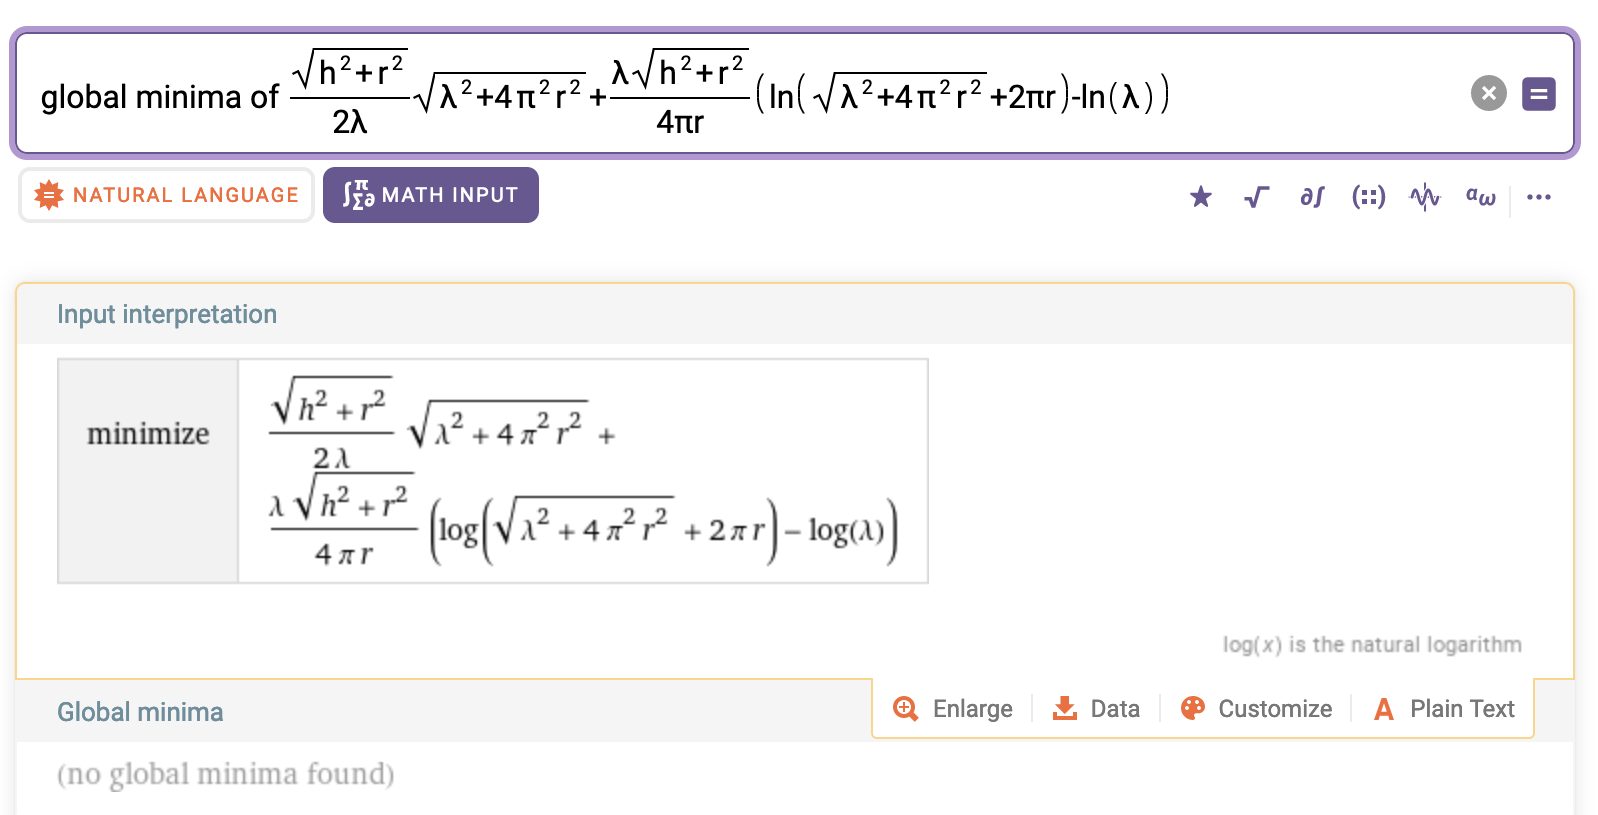
\includegraphics[width=\textwidth]{images/wolfram_global_minima.png}
    \end{subfigure}
\end{figure}
\begin{figure}[H]\ContinuedFloat
    \centering
    \begin{subfigure}[t]{0.7\textwidth}
        \centering
        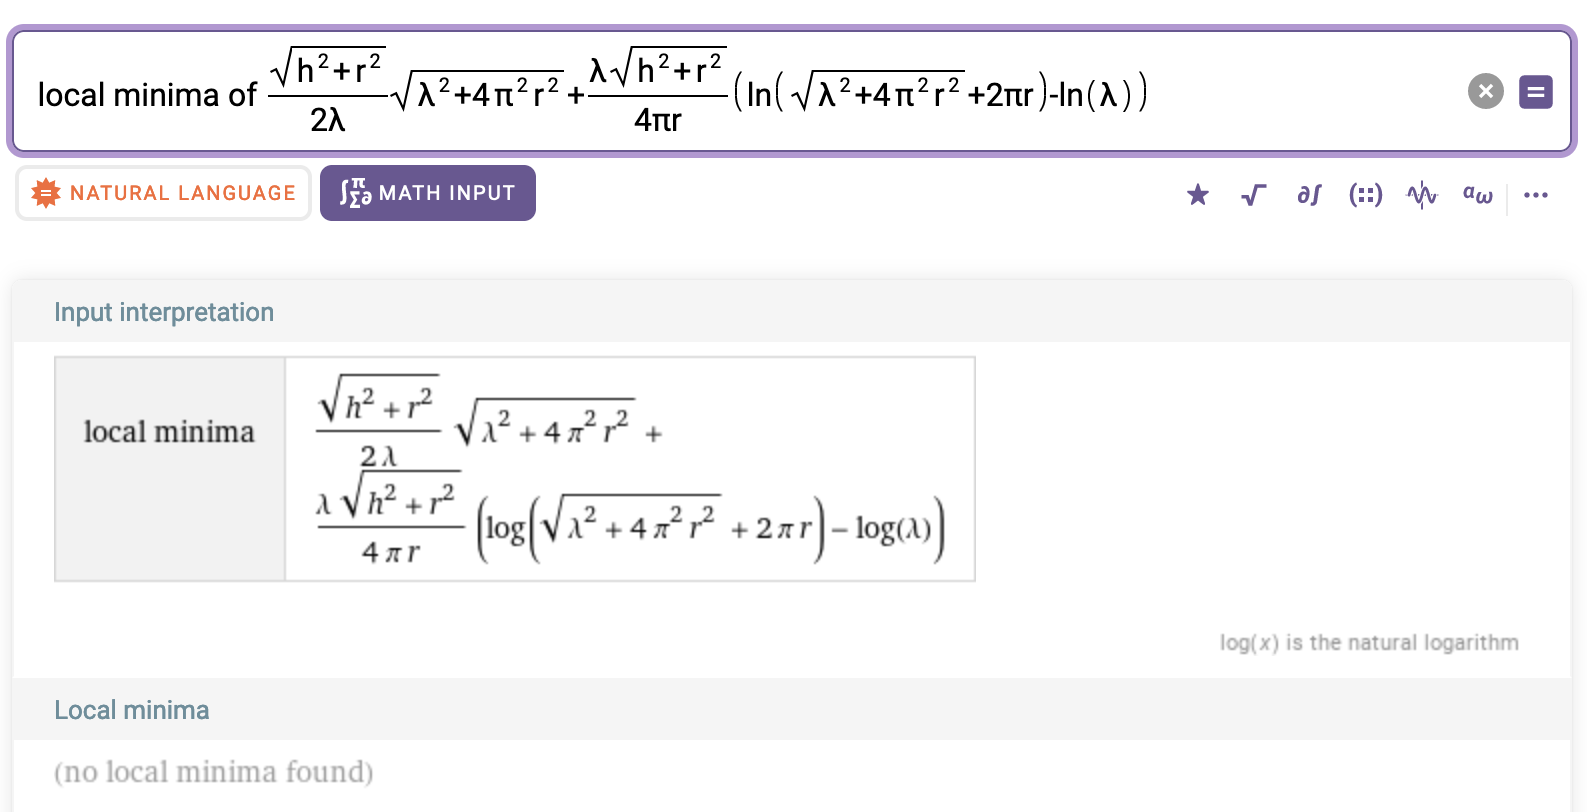
\includegraphics[width=\textwidth]{images/wolfram_local_minima.png}
    \end{subfigure}
    \caption{The equation has no global or local minima, according to \emph{Wolfram Alpha}.}
    \vspace*{-10pt}
\end{figure}

Given that there are no globally optimal solutions, I decided that I should instead focus on my particular Christmas tree, which has the dimensions $R=\US{15}{\inch}$ and $H=\US{72}{\inch}$. I realized it was important to first understand the dynamics of the function, and so I graphed the function in \emph{Desmos}, with $\lambda$ as the independent variable and $L$ as the dependent variable, as visualized in Figure \ref{fig:graph}. Firstly, I noted that the function was decreasing over the entire domain, meaning that as $\lambda$ increases, the length of garland required $L$ decreases. This is reasonable, given that larger spacing between successive rotations of the garland would mean that garland would have to go around the tree a lesser amount of times before it reaches to the tip of the tree, and thus mean that a shorter length of garland is necessary.
\begin{figure}[H]
    \vspace*{5pt}
    \centering
    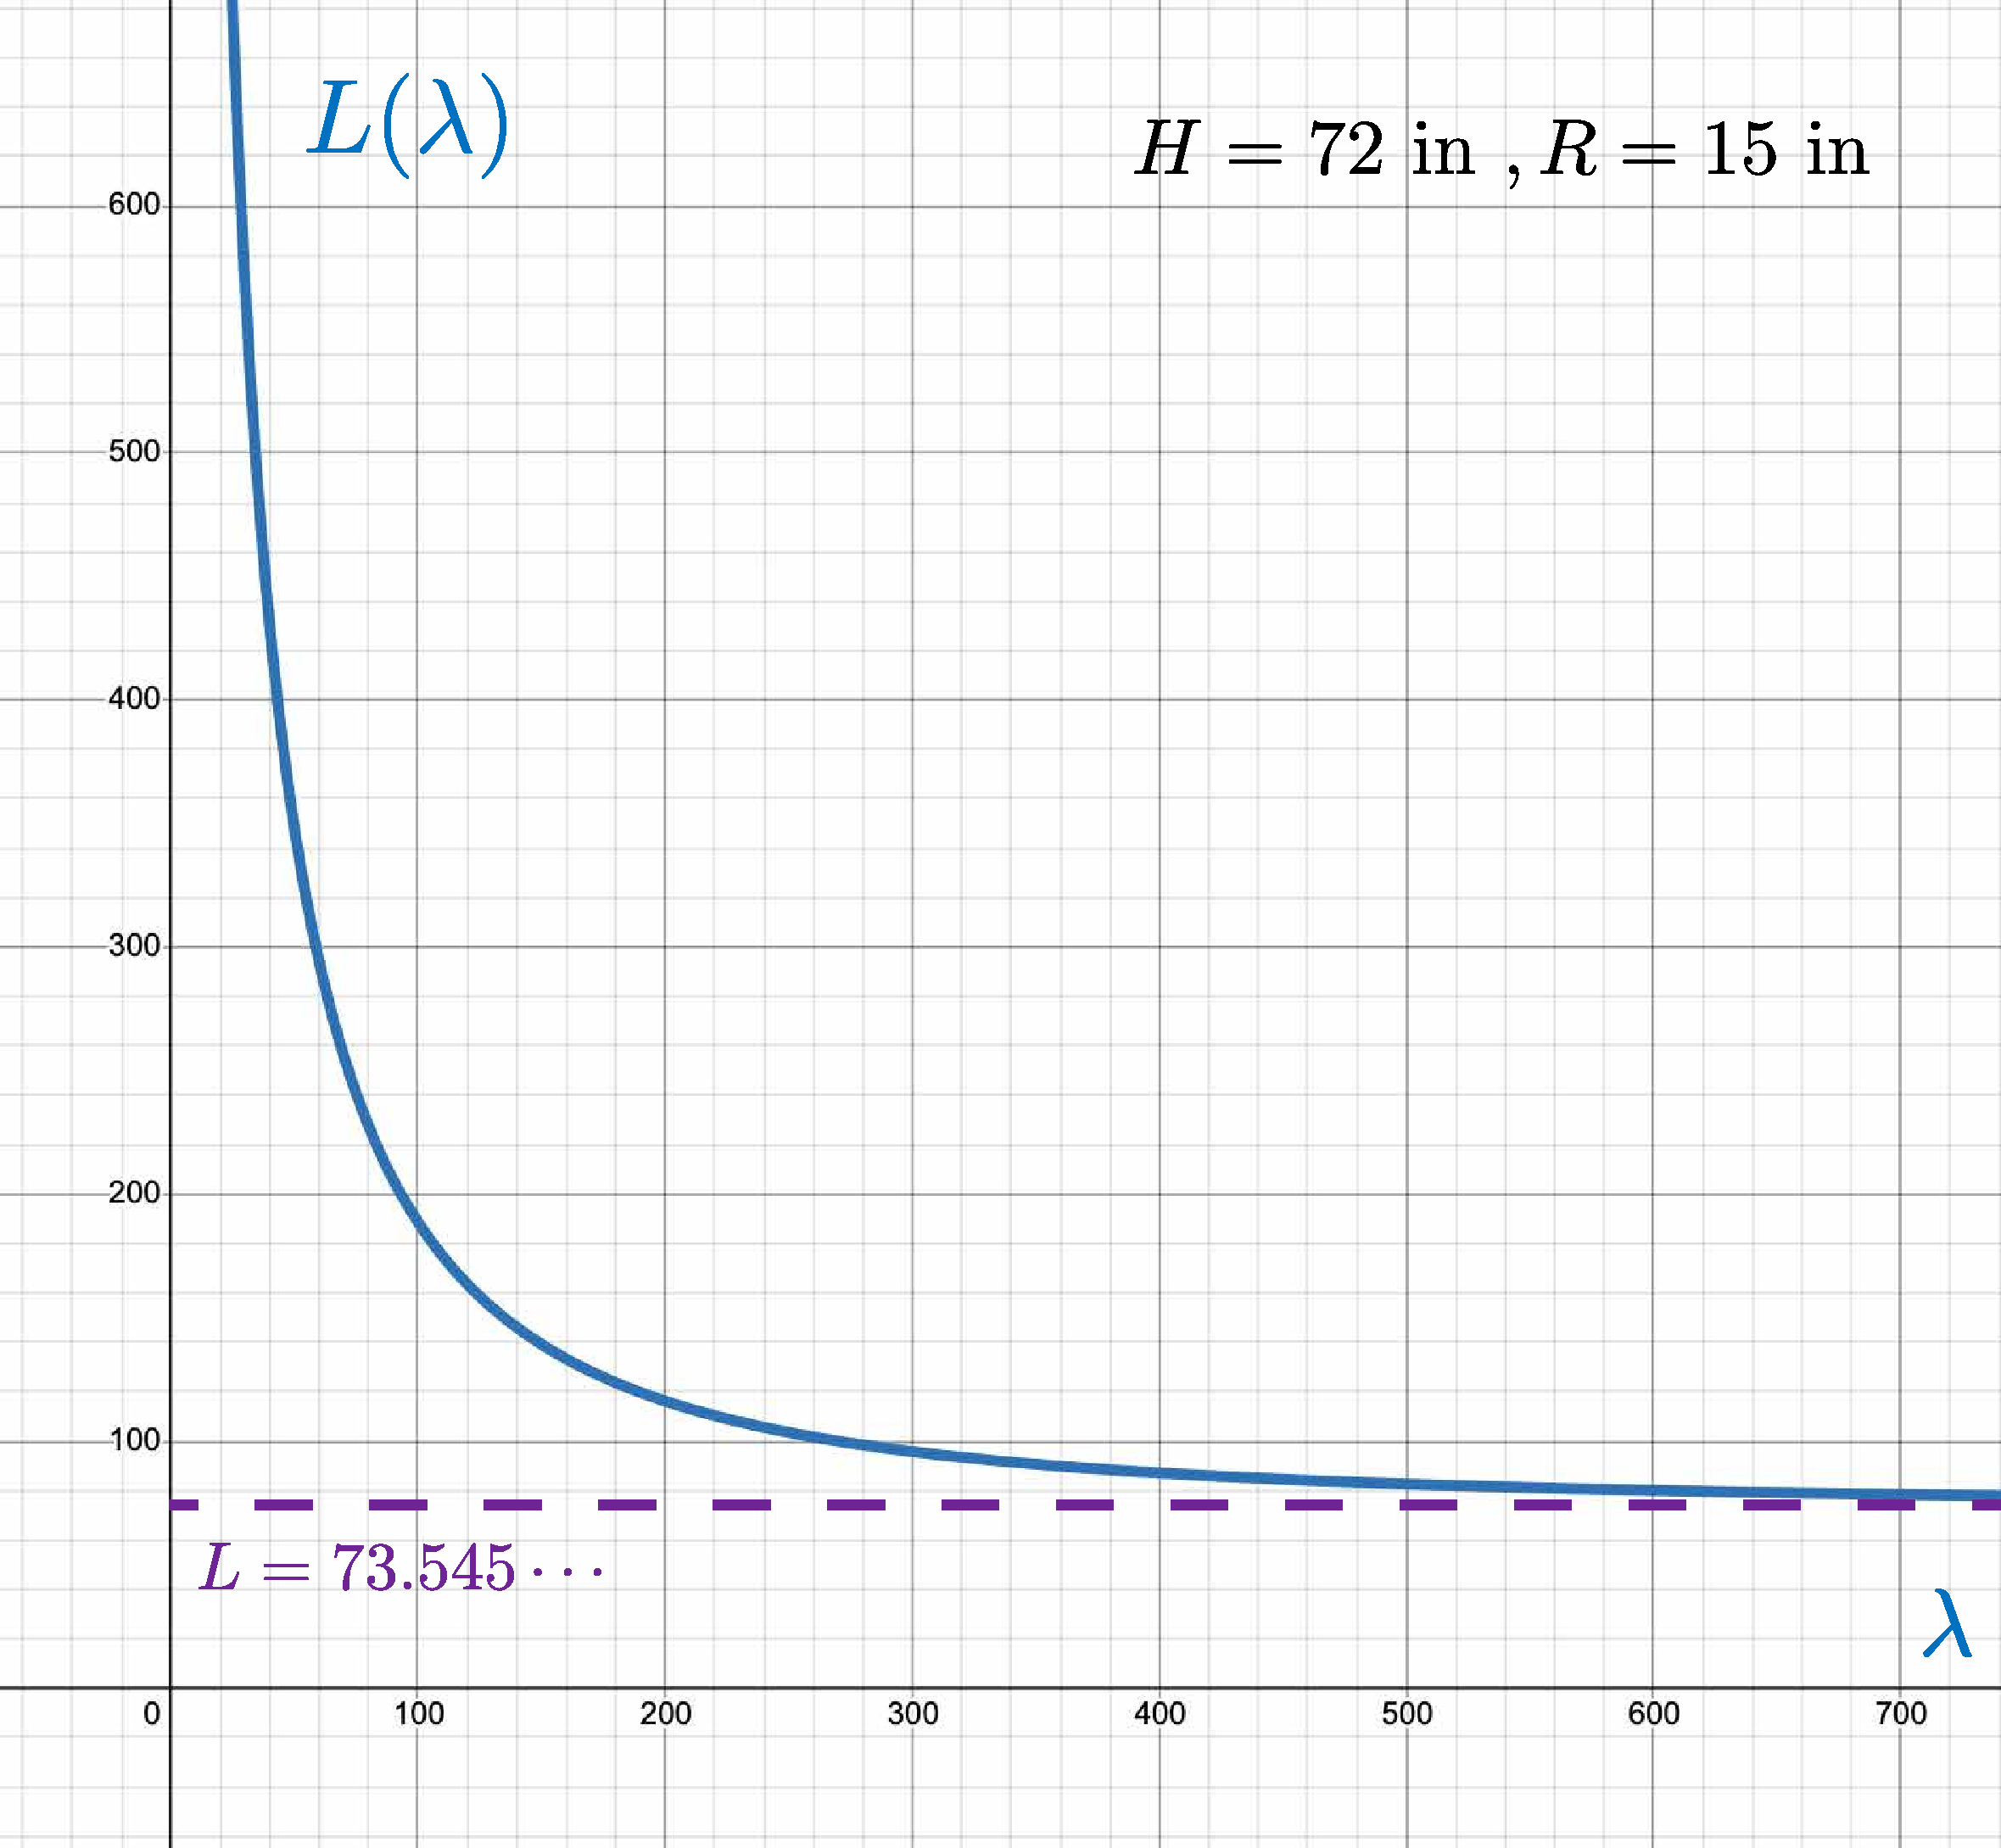
\includegraphics[width=0.6\textwidth]{diagrams/graph.pdf}
    \caption{Graph of $L$ vs. $\lambda$ with $H=\US{72}{\inch}$ and $R=\US{15}{\inch}$} \label{fig:graph}
    \vspace*{-15pt}
\end{figure}
\noindent Another interesting thing to note is that the function is asymptotic, because from the graph we can see that as $\lambda \rightarrow +\infty$, $L$ converges towards $L = \US{73.5459}{\inch}$, which is the slant height of the cone ($\sqrt{15^2+72^2} = 73.5459\cdots$). In fact, it is true for all values of $R, H \in \Real^+$ that $\dss\lim_{\lambda \to +\infty} L(\lambda, R, H) = \sqrt{R^2+H^2}$, which is the slant height $S$ of the tree (see Appendix \ref{sec:qzhsb} for the full derivation of the limit). This makes sense, given that the shortest length possible for the garland would be a straight line from the tip of the tree to the bottom of the tree, which would be equal to the slant height. Finally, we see that as $\lambda \to 0$ from the right, $L$ exponentially increases and diverges towards $+\infty$. Thus, while I want to space the garland such that the tree look nice according to my personal preferences, it is also important not to choose a spacing too small, as it would require a lot more garland, and not only is that wasteful and unnecessary spending, it is harmful to the environment as I will be using plastic tinsel garland.

Since we established above that the function does not have minima, I will have to add further constraints in order to arrive at ``optimal'' solution(s). One thing I quickly realized was that the function is continuous, but the reality is that garland is typically sold in standard unit lengths; for example, the garland which my family bought is sold in $\US{6}{\feet}$ strands (or $\US{72}{\inch}$). This means that the amount of garland that I buy can only be a positive multiple of unit lengths of garland, which can mathematically represented thus:
\begin{equation}
    L_G = nG,\quad n \in \Integer^+ \label{eq:nG}
\end{equation}
where $L_G$ denotes the total length of garland required, $G$ represents the individual unit of a strand of garland, and $n\in \Integer^+$ is the number of strands of garland that I need to buy. As such, the function which computes the amount of garland required should really be modelled as a step function, and if I wanted to minimize the amount of garland wasted by having as little excess garland as possible, I would want the theoretical minimum amount of garland, $L$, to be roughly equal to some multiple of $G$, i.e. $L(\lambda, R, H) = nG$.

My initial approach to solving this problem was to find a way to isolate for $\lambda$, which would basically allow me to have $\lambda$ as a function of $n$. This would be very useful, as I could input positive integers into $n$ and generate all possible values for $\lambda$ which result in lengths of the garland that are multiples of $G$. However, I quickly realized that this was not viable, as the complexity of my formula from the square roots and the logarithms means that it is very difficult or most likely impossible to isolate for $\lambda$. As such, this problem will have to be approached in a numerical manner. Given that I already have my formula that solves for the length of garland necessary, I can find the number of lengths of garland that I need to buy to cover that length, $n$, by dividing that length by the unit lengths of a strand garland, $G$, and rounding up the result to the next whole number. This can be mathematically represented using the ceiling function:
\begin{equation}
    n = \left\lceil \frac{L(\lambda, R, H)}{G} \right\rceil
\end{equation}
Plugging this back into equation \ref{eq:nG}, we get that:
\begin{equation}
    L_G = G\left\lceil \frac{L(\lambda, R, H)}{G} \right\rceil
\end{equation}
Then, using \emph{Desmos}, I generated a graph which compares $L$ to $L_G$ (Figure \ref{fig:LG}).

\begin{figure}[H]
    \centering
    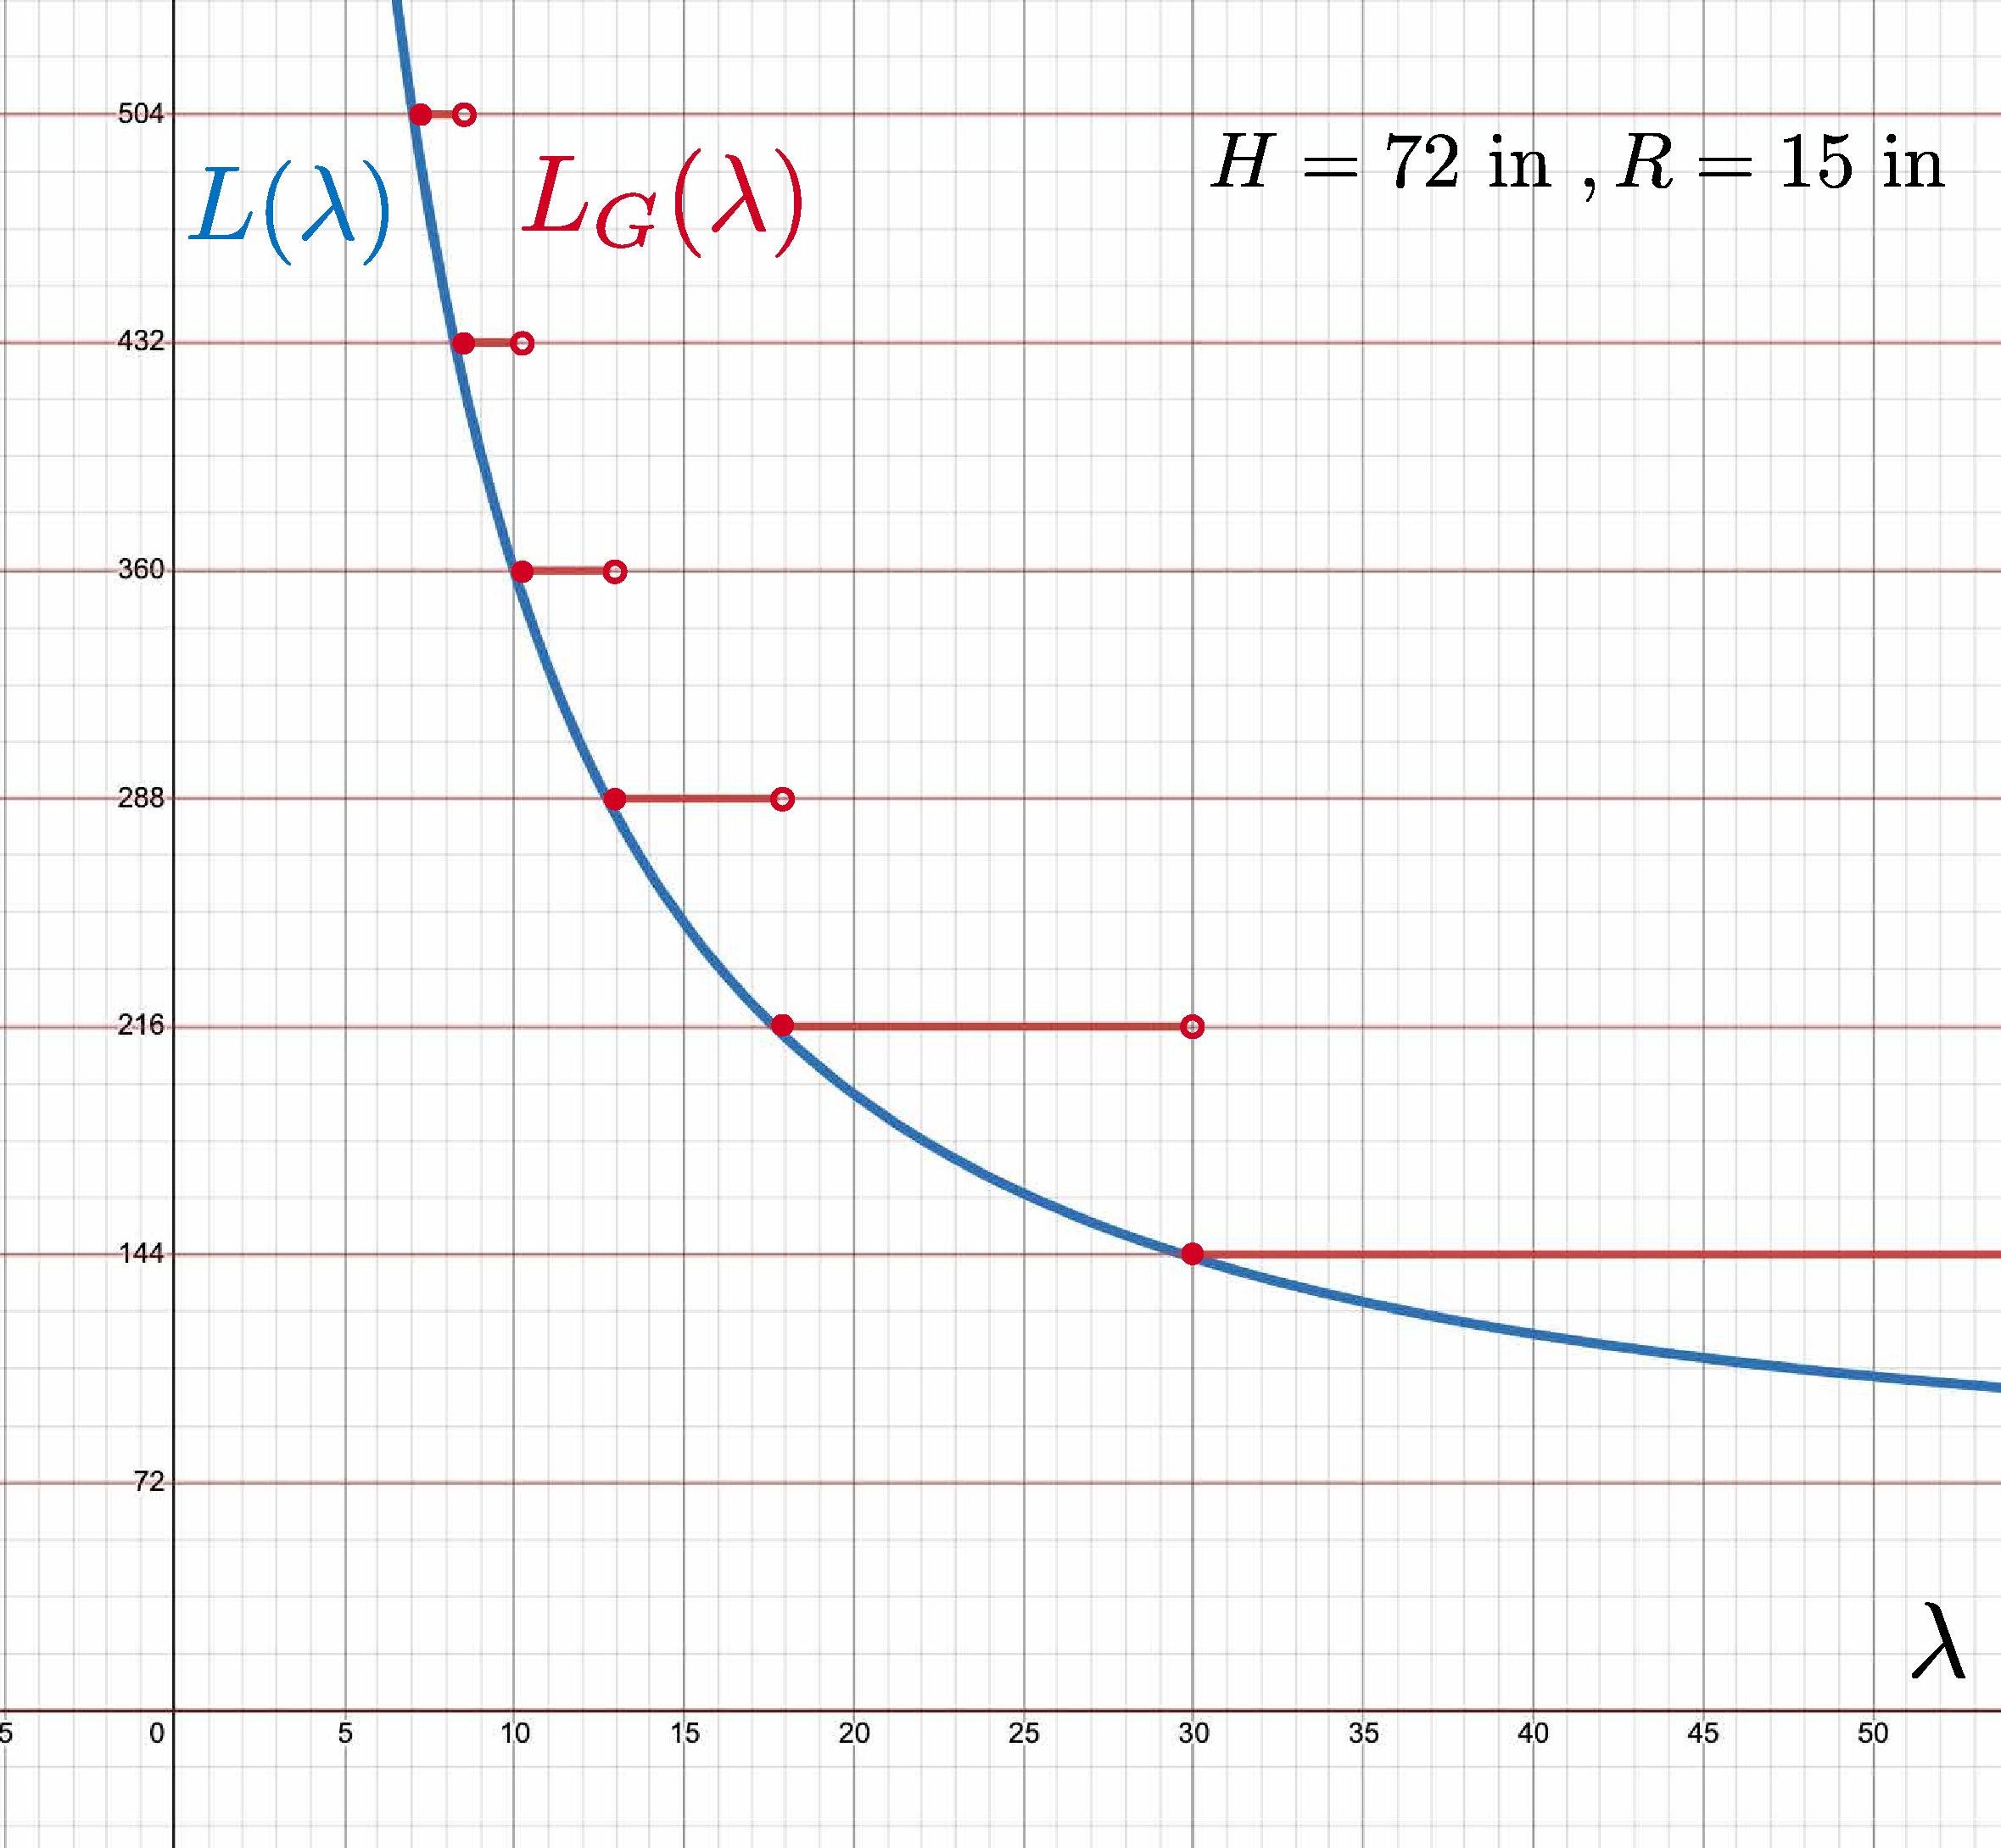
\includegraphics[width=0.6\textwidth]{diagrams/step_comparison.pdf}
    \caption{A comparison between $L$ and $L_G$.} \label{fig:LG}
\end{figure}

Graphically, we can see that solutions for $\lambda$ which does not waste any garland would be where $L$ intersects $L_G$. However, such values of $\lambda$ will almost certainly be too precise -- it is often the case that optimal solutions do not yield ``nice'' or expressible numbers, such as irrational numbers. We want practical solutions where the spacing is a number that is easy to work with. It is also important to consider the unit of measurement to use; given that measurements for Christmas trees are typically expressed in feet in my country of origin, I opted to use inches for my investigation. Note that metric units (such as the meter) use decimal subdivisions, while imperial units, particularly the inch, is usually subdivided using fractions (generally powers of 2). Since I will be using the inch as my unit of measurement, I decided that for practical purposes I would limit the precision of $\lambda$ to a \sfrac{1}{4} of an inch. Implementing this new restriction, I generated a table of values (see Appendix \ref{sec:table}), and graphed the data points using \emph{Google Sheets}.

\begin{figure}[H]
    \centering
    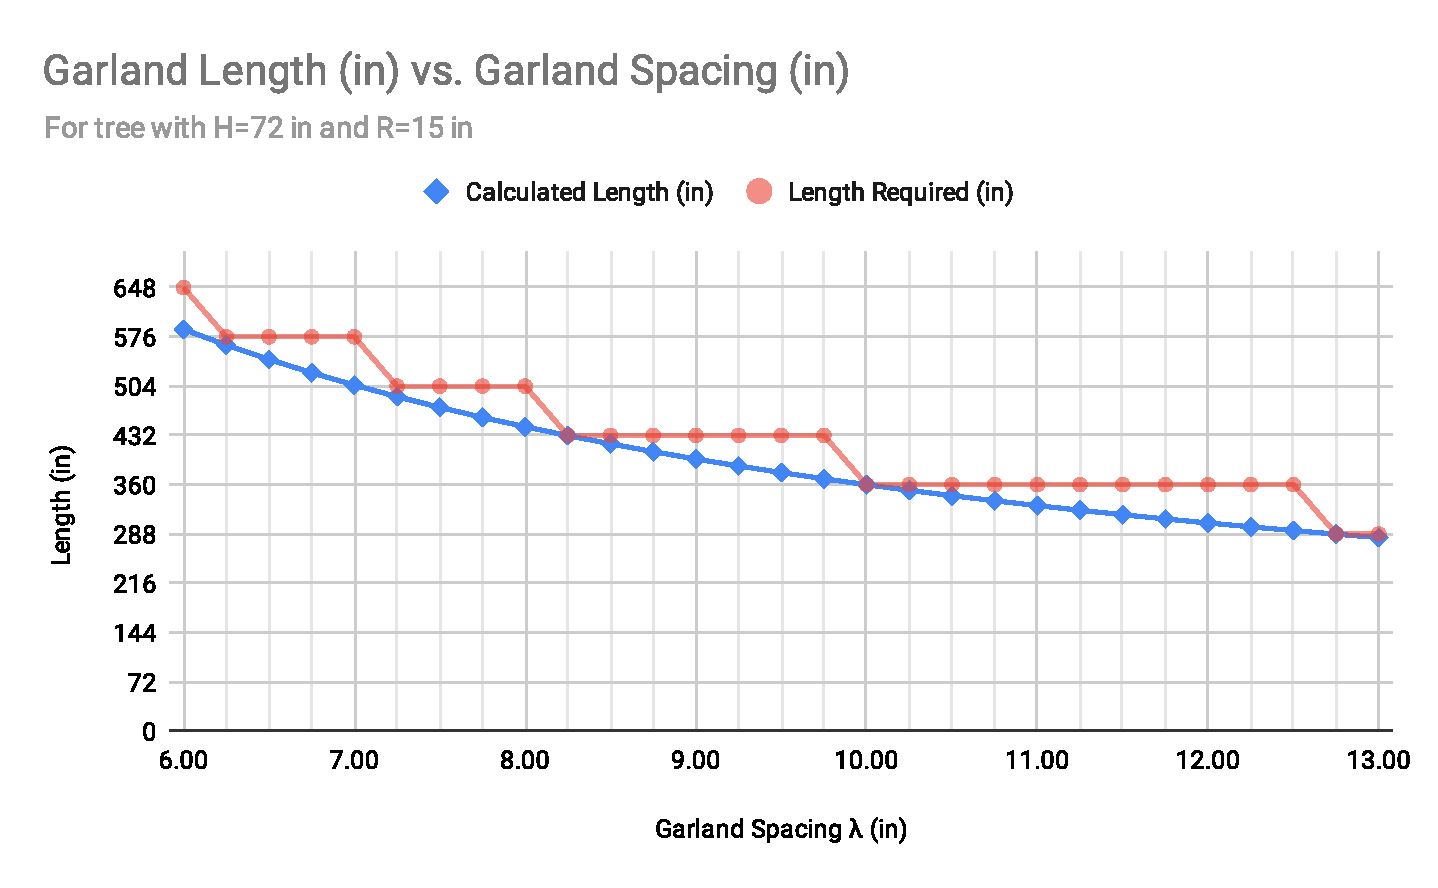
\includegraphics[width=0.9\textwidth]{diagrams/detailed_graph.pdf}
    \caption{Graph showing the length of garland $L$ vs. the garland spacing $\lambda$, at \sfrac{1}{4} $\unit{\inch}$ intervals. (Generated using \emph{Google Sheets})} \label{fig:detailed}
\end{figure}

We have thus narrowed down the dataset of potential solutions, and by performing the calculation $L_G-L$, we can find the amount garland that is wasted, and weed out solutions which waste too much garland. But the problem is -- how much wasted garland is too much?  Ultimately, this is again a subjective problem, and depending on how loose or strict this restriction is, we will get either more or less prospective answers. Arbitrarily, I will set my cutoff to be 15\% of the unit length of garland, or $\US{10.8}{\inch}$.  Under these new criteria, there are 5 values of $\lambda$ between $\lambda=\US{6}{\inch}$ and $\lambda=\US{13}{\inch}$ that fit these criteria -- $\qtylist{8.25;10.00;10.25;12.75;13.00}{\inch}$.

\begin{table}[H]
    \centering
    \singlespacing
    \setlength{\tabcolsep}{10pt}
    \resizebox{\textwidth}{!}{
        \begin{tabular}{ccccc}
            \toprule
            \textbf{Spacing ($\lambda$)} & \textbf{Min. Length ($L$)} & \textbf{\# of Garland} & \textbf{Length To Buy ($L_G$)} & \textbf{Excess Garland} \\
            \midrule
            10.00                        & 359.99                     & 5                      & 360                            & 0.01                    \\
            8.25                         & 431.78                     & 6                      & 432                            & 0.22                    \\
            12.75                        & 287.72                     & 4                      & 288                            & 0.28                    \\
            13.00                        & 282.71                     & 4                      & 288                            & 5.29                    \\
            10.25                        & 351.77                     & 5                      & 360                            & 8.23                    \\
            \bottomrule
        \end{tabular}
    }
    \caption{Values of $\lambda$ and associated computations, with less than $\US{12}{\inch}$ of excess garland.  All values below are measured in \textbf{inches} and sorted by amount of excess garland in increasing order}
\end{table}

Now that I have found answers which satisfy my first aim of minimizing waste, I now want to consider answers which result in the Christmas tree looking the best according to my own opinions. Looking at various blogs on decorating Christmas trees, such as \citeauthor{rooneyHowString2019}'s \citetitle{rooneyHowString2019}, they recommend having the garland spaced at $\US{1}{\feet}$ ($\US{12}{\inch}$) from each other. However, when modelling trees with garland of varying values of $\lambda$ using \emph{Desmos} and comparing how they looked, I found that I personally liked the garland spaced closer to each other, with garland spaced between $\qtyrange{8.00}{10.00}{\inch}$ looking the best. Anything below my lower limit looked overly dense, while anything over the upper limit looked too bare and needed more garland. 

\begin{figure}[H]
    \centering
    \begin{subfigure}[t]{0.2\textwidth}
        \centering
        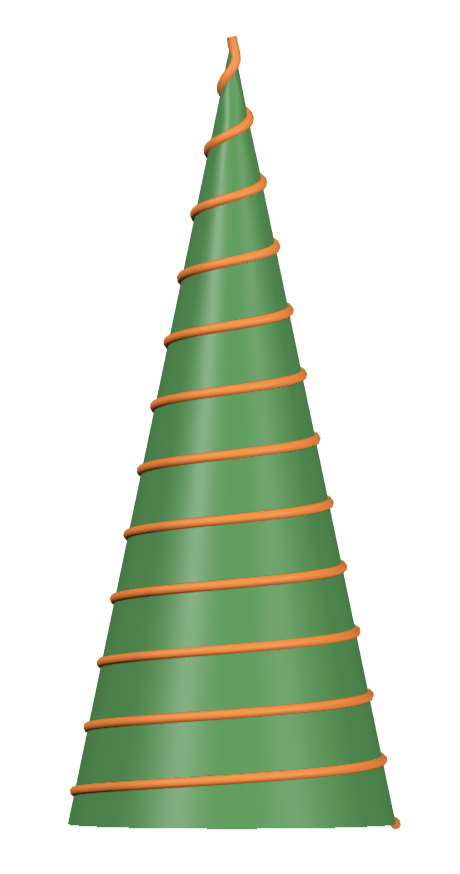
\includegraphics[width=\textwidth]{images/garland_spacings/6in.png}
        \caption{$\US{6}{\inch}$ Spacing.}
    \end{subfigure}
    \hspace*{0.05\textwidth}
    \begin{subfigure}[t]{0.2\textwidth}
        \centering
        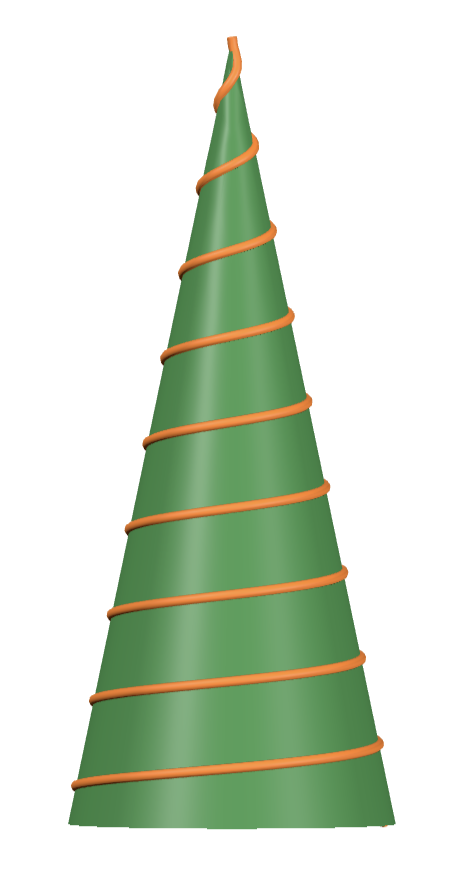
\includegraphics[width=\textwidth]{images/garland_spacings/8in.png}
        \caption{$\US{8}{\inch}$ Spacing.}
    \end{subfigure}
    \hspace*{0.05\textwidth}
    \begin{subfigure}[t]{0.2\textwidth}
        \centering
        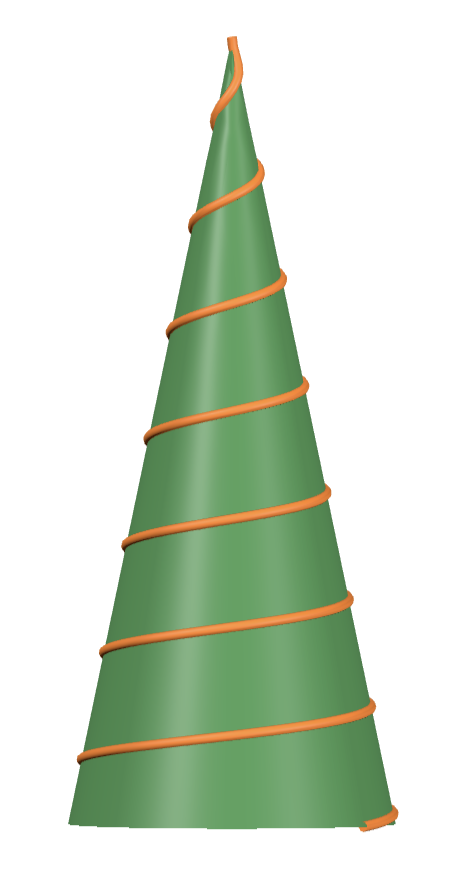
\includegraphics[width=\textwidth]{images/garland_spacings/10in.png}
        \caption{$\US{10}{\inch}$ Spacing.}
    \end{subfigure}
    \hspace*{0.05\textwidth}
    \begin{subfigure}[t]{0.2\textwidth}
        \centering
        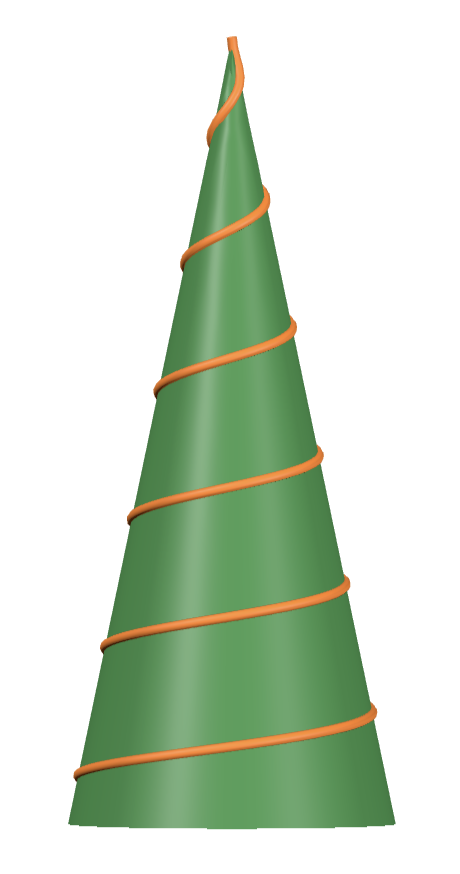
\includegraphics[width=\textwidth]{images/garland_spacings/12in.png}
        \caption{$\US{12}{\inch}$ Spacing.}
    \end{subfigure}
    \caption{Comparison between different spacing for the garland. }
\end{figure}

Finally, there are only 2 values of $\lambda$ which satisfies all the criteria that I set out. The values are $\lambda=\US{8.25}{\inch}$ and $\lambda=\US{10.00}{\inch}$. Ultimately, I chose $\boxed{\mathbf{\lambda=\US{10.00}{\inch}}}$, because it uses 5 strands of garland as opposed to 6, and minimizing waste is a more important priority to me compared to aesthetics. 

\section{Conclusion and Evaluation}

In this investigation, I was successful in deriving a formula which calculates the length of garland required to wrap around my Christmas tree based on the spacing between successive rotations of garland $\lambda$, the base radius of the tree $R$, and the height of the tree $H$. This was done by modelling the garland as a circular conical spiral, and by finding the arc length of the spiral using integration, I was able to find the approximate length garland I would need based on my chosen parameters. Then, I applied this formula by plugging in the dimensions of my tree, and found optimal values of $\lambda$ by only considering solutions precise up to a \sfrac{1}{4} of an inch, and subjected the function to further constraints -- the amount of wasted garland must be less than 15\% of the length of a strand of garland ($\US{12}{\inch}$), and potential values of $\lambda$ must be between $\qtyrange{8.00}{10.00}{\inch}$. I selected these two constraints rather arbitrarily to satisfy each of my respective aims: minimizing waste and aligning with my personal aesthetic preferences. There were two solutions which met these constraints, and I ultimately chose $\lambda=\US{10}{\inch}$, requiring the use of 5 strands of garland that are $\US{72}{\inch}$ long, totaling in $\US{360}{\inch}$ or $\US{30}{\feet}$ of garland. 

While I was able to meet all of my objectives in my investigation and find an ``optimal'' answer, it is also important to realize that my investigation was hinged upon the two big assumptions that I made in the beginning of my investigation -- that the tree can be modelled as a cone, and that the garland wraps the cone perfectly as a circular conical spiral. In reality, trees will always have imperfections, and the garland will sag as it travels up the tree. It is also difficult to account for how each person wraps the garland around the tree differently, as some people may wrap the garland more tightly around the tree, while others may wrap it around looser. These differences can add up, leading to large variations in the amount of garland used, and considering that I chose a solution which had effectively no remaining excess garland ($\US{0.01}{\inch}$), there is very little room for error. The formula is also rather complex, meaning that it is not really accessible to those who are not mathematically inclined. As such, I can make my formula more accessible by approximating it using simpler functions, as well as potentially accounting for some leeway (such as by including a scale factor), as it would be better to have an overestimation rather than an underestimation. An assessment of how this might be achieved can be a possible extension to this study.


\label{lastpage}

% ==================

%TC:ignore
\clearpage
\pagestyle{references}
\printbibliography[heading=bibintoc]{}

% ==================
\clearpage
\pagestyle{appendices}
\titleformat{\section}{\normalfont\normalsize\bfseries}{\thesection}{1em}{}
\begin{appendices}
    \section{Calculated Table for My Christmas Tree} \label{sec:table}

The calculations in the table below are for a Christmas tree with base radius $R=\US{15}{\inch}$ and height $H=\US{72}{\inch}$. The unit length of the garland is $G=\US{72}{\inch}$. Note that all values below are measured in \textbf{inches}.
\begin{table}[H]
    \centering
    \singlespacing
    \setlength{\tabcolsep}{10pt}
    \resizebox{\textwidth}{!}{
        \begin{tabular}{ccccc}
            \toprule
            \textbf{Spacing ($\lambda$)} & \textbf{Min. Length ($L$)} & \textbf{\# of Garland} & \textbf{Length To Buy ($L_G$)} & \textbf{Excess Garland} \\
            \midrule
            6.00                         & 586.87                     & 9                      & 648                            & 61.13                   \\
            6.25                         & 564.05                     & 8                      & 576                            & 11.95                   \\
            6.50                         & 543.00                     & 8                      & 576                            & 33.00                   \\
            6.75                         & 523.53                     & 8                      & 576                            & 52.47                   \\
            \\
            7.00                         & 505.47                     & 8                      & 576                            & 70.53                   \\
            7.25                         & 488.67                     & 7                      & 504                            & 15.33                   \\
            7.50                         & 473.00                     & 7                      & 504                            & 31.00                   \\
            7.75                         & 458.36                     & 7                      & 504                            & 45.64                   \\
            \\
            8.00                         & 444.65                     & 7                      & 504                            & 59.35                   \\
            8.25                         & 431.78                     & 6                      & 432                            & 0.22                    \\
            8.50                         & 419.68                     & 6                      & 432                            & 12.32                   \\
            8.75                         & 408.28                     & 6                      & 432                            & 23.72                   \\
            \\
            9.00                         & 397.53                     & 6                      & 432                            & 34.47                   \\
            9.25                         & 387.37                     & 6                      & 432                            & 44.63                   \\
            9.50                         & 377.75                     & 6                      & 432                            & 54.25                   \\
            9.75                         & 368.64                     & 6                      & 432                            & 63.36                   \\
            \\
            10.00                        & 359.99                     & 5                      & 360                            & 0.01                    \\
            10.25                        & 351.77                     & 5                      & 360                            & 8.23                    \\
            10.50                        & 343.96                     & 5                      & 360                            & 16.04                   \\
            10.75                        & 336.51                     & 5                      & 360                            & 23.49                   \\
            \\
            11.00                        & 329.42                     & 5                      & 360                            & 30.58                   \\
            11.25                        & 322.64                     & 5                      & 360                            & 37.36                   \\
            11.50                        & 316.17                     & 5                      & 360                            & 43.83                   \\
            11.75                        & 309.98                     & 5                      & 360                            & 50.02                   \\
            \\
            12.00                        & 304.06                     & 5                      & 360                            & 55.94                   \\
            12.25                        & 298.39                     & 5                      & 360                            & 61.61                   \\
            12.50                        & 292.94                     & 5                      & 360                            & 67.06                   \\
            12.75                        & 287.72                     & 4                      & 288                            & 0.28                    \\
            \bottomrule
        \end{tabular}
    }
\end{table}

    \section{Solving the Limit of $L(\lambda, R, H)$ as $\lambda \to +\infty$} \label{sec:qzhsb}

\begin{align*}
     \lim_{\lambda \to +\infty} &\left(\frac{\sqrt{R^2+H^2}}{2\lambda}\sqrt{\lambda^2+4\pi^2R^2}+\frac{\lambda \sqrt{R^2+H^2}}{4\pi R}\bigg[\ln\left(\sqrt{\lambda^2+4\pi^2R^2}+2\pi R\right)-\ln\lambda\bigg]\right) \\ 
    &= \lim_{\lambda \to +\infty} \frac{\sqrt{R^2+H^2}}{2\lambda}\sqrt{\lambda^2+4\pi^2R^2}+ \lim_{\lambda \to +\infty}\frac{\lambda \sqrt{R^2+H^2}}{4\pi R}\bigg[\ln\left(\sqrt{\lambda^2+4\pi^2R^2}+2\pi R\right)-\ln\lambda\bigg] \\ 
    &= \lim_{\lambda \to +\infty} \frac{\cancel{\lambda}\sqrt{R^2+H^2}}{2\cancel{\lambda}} \cdot \cancelto{1}{\lim_{\lambda \to +\infty} \sqrt{1+\frac{4\pi^2R^2}{\lambda^2}}} + \lim_{\lambda \to +\infty}\frac{\lambda \sqrt{R^2+H^2}}{4\pi R}\bigg[\ln\left(\sqrt{\lambda^2+4\pi^2R^2}+2\pi R\right)-\ln\lambda\bigg] \\
    &=\frac{\sqrt{R^2+H^2}}{2} + \lim_{\lambda \to +\infty} \frac{\ln\left(\sqrt{\lambda^2+4\pi^2R^2}+2\pi R\right)-\ln\lambda}{\frac{4\pi R}{\lambda \sqrt{R^2+H^2}}} \\
\intertext{\bulletarrow{Since the limit of the second term evaluates to $\frac{0}{0}$, by l'H\^{o}pital's rule:}}
    &= \frac{\sqrt{R^2+H^2}}{2} + \lim_{\lambda \to +\infty} \frac{\dv{\lambda}\left(\ln\left(\sqrt{\lambda^2+4\pi^2R^2}+2\pi R\right)-\ln\lambda\right)}{\dv{\lambda}\left(\frac{4\pi R}{\lambda \sqrt{R^2+H^2}}\right)} \\ 
    &= \frac{\sqrt{R^2+H^2}}{2} + \lim_{\lambda \to +\infty} \frac{\frac{-1}{\lambda}+\frac{\lambda}{2\pi R\sqrt{\lambda^2+4\pi^2R^2}+4\pi^2R^2+\lambda^2}}{\frac{-4\pi R}{\lambda^2\sqrt{R^2+H^2}}} \\ 
\intertext{\bulletarrow{Combining the fractions in the limit by taking the common denominator:}}
    &= \frac{\sqrt{R^2+H^2}}{2} + \lim_{\lambda \to +\infty} \left(\frac{-\lambda^2\sqrt{R^2+H^2}}{4\pi R} \cdot \frac{\cancel{\lambda^2}-2\pi R\sqrt{\lambda^2+4\pi^2R^2}-4\pi^2R^2\cancel{-\lambda^2}}{2\pi R\lambda\sqrt{\lambda^2+4\pi^2R^2}+4\pi^2R^2\lambda+\lambda^3}\right) \\
    &= \frac{\sqrt{R^2+H^2}}{2} + \lim_{\lambda \to +\infty} \left(\frac{\lambda^2\sqrt{R^2+H^2}}{4\pi R} \cdot \frac{2\pi R\lambda\sqrt{1+\frac{4\pi^2R^2}{\lambda^2}}+4\pi^2R^2}{2\pi R\lambda^2\sqrt{1+\frac{4\pi^2R^2}{\lambda^2}}+4\pi^2R^2\lambda+\lambda^3}\right) \\ 
\intertext{\bulletarrow{Multiplying the numerator and denominator by $\frac{1}{\lambda^3}$:}}
    &= \frac{\sqrt{R^2+H^2}}{2} + \lim_{\lambda \to +\infty} \left(\frac{\sqrt{R^2+H^2}}{4\pi R} \cdot \frac{2\pi R\sqrt{1+\frac{4\pi^2R^2}{\lambda^2}}+\frac{4\pi^2R^2}{\lambda}}{\frac{2\pi R\sqrt{1+\frac{4\pi^2R^2}{\lambda^2}}}{\lambda}+\frac{4\pi^2R^2}{\lambda^2}+1}\right) \\ 
    &= \frac{\sqrt{R^2+H^2}}{2} + \frac{\sqrt{R^2+H^2}}{2} \cdot \cancelto{1}{\lim_{\lambda \to +\infty} \frac{\sqrt{1+\frac{4\pi^2R^2}{\lambda^2}}+\frac{2\pi R}{\lambda}}{\frac{2\pi R\sqrt{1+\frac{4\pi^2R^2}{\lambda^2}}}{\lambda}+\frac{4\pi^2R^2}{\lambda^2}+1}} \\ 
    &\boxed{=\sqrt{R^2+H^2}}
\end{align*}
Thus, the limit of $L(\lambda, R. H)$ as $\lambda \to +\infty$ will always be equal to the slant height of the tree.

\end{appendices}
%TC:endignore


\end{document} % END

